% Documentacion del proyecto GGEZ. Compilar desde docs/ con: xelatex documentacion.tex (dos veces)
% Las tablas de la seccion 18 salen de: python Traductor/pruebas/correr.py --latex docs/pruebas_tablas.tex
% Preambulo comun de documentacion.tex y manual_usuario.tex
\documentclass[11pt,a4paper]{article}

\usepackage{fontspec}
\usepackage{polyglossia}
\setmainlanguage{spanish}
\setmainfont{Liberation Serif}
\setmonofont{Liberation Mono}[Scale=0.9]
\usepackage[margin=2.5cm]{geometry}
\usepackage[table]{xcolor}
\usepackage{graphicx,fancyhdr,longtable,array,listings,caption,float}
\usepackage[hidelinks]{hyperref}
\Urlmuskip=0mu plus 2mu\def\UrlBreaks{\do\/\do-\do.}

\setlength{\parskip}{0.7em}
\setlength{\parindent}{0pt}
\setlength{\emergencystretch}{2em}
\linespread{1.15}
\renewcommand{\arraystretch}{1.2}

% "1. Introduccion" con punto solo en las secciones; "3.1 Titulo" sin punto
\makeatletter
\def\@seccntformat#1{\csname the#1\endcsname\csname punto@#1\endcsname\quad}
\def\punto@section{.}
\makeatother
\addto\captionsspanish{\renewcommand{\contentsname}{Tabla de contenidos}}

% "Pagina X de Y" sin el paquete lastpage
\AtEndDocument{\label{ultimapagina}}
\pagestyle{fancy}
\fancyhf{}
\renewcommand{\headrulewidth}{0pt}
\fancyfoot[C]{\small Página \thepage\ de \pageref{ultimapagina}}

\newcommand{\kw}[1]{\texttt{#1}}
\newcommand{\ggez}{GGEZ}

\lstdefinelanguage{GGEZ}{
  sensitive=true,
  morecomment=[l]{/w},
  morecomment=[s]{/all}{/end},
  morestring=[b]",
}
\lstset{
  language=GGEZ, basicstyle=\ttfamily\small, columns=fullflexible, keepspaces=true,
  breaklines=true, showstringspaces=false, xleftmargin=1.2em, aboveskip=0.4em, belowskip=0.6em,
}

% Tablas al estilo del documento: encabezado gris y filas de categoria
\newcommand{\cab}{\rowcolor{gray!22}}
\newcommand{\categoria}[2]{\multicolumn{#1}{|l|}{\cellcolor{gray!10}\textbf{#2}}\\\hline}

% Tabla de pruebas: la generan Traductor/pruebas/correr.py
\newenvironment{tablaprueba}{\footnotesize
  \begin{longtable}{|p{3.4cm}|p{3.0cm}|p{5.6cm}|p{2.1cm}|}\hline
  \cab\textbf{Prueba y objetivo} & \textbf{Entrada} & \textbf{Resultado esperado} & \textbf{Resultado obtenido y estado}\\\hline\endhead}
  {\end{longtable}}


\begin{document}

% ---------------------------------------------------------------- Portada
\thispagestyle{empty}
\begingroup\setlength{\parskip}{0pt}
\begin{center}
\vspace*{0.5cm}
{\bfseries UNIVERSIDAD NACIONAL\par}
\vspace{0.4cm}
{\bfseries SEDE REGIONAL BRUNCA -- CAMPUS PÉREZ ZELEDÓN\par}
\vspace{0.4cm}
{CURSO: PARADIGMAS DE PROGRAMACIÓN\par}
\vspace{1cm}

\includegraphics[width=3.6cm]{img/una.png}\par
\vspace{1.2cm}
{\large\bfseries PROYECTO FINAL\par}
\vspace{0.6cm}
{\large\textbf{GGEZ}: \emph{Lenguaje de programación con vocabulario de videojuegos para estudiantes de primer ingreso}\par}
\vspace{0.8cm}

\includegraphics[width=3.2cm]{img/logo.png}\par
\vspace{1cm}
{\bfseries Integrantes:\par}
\vspace{0.3cm}
Steven Mata Quirós\par\vspace{0.2cm}
Maikel Segura Quirós\par\vspace{0.2cm}
Angel Ureña Naranjo\par
\vspace{0.8cm}
{\bfseries Profesor:\par}
\vspace{0.3cm}
Pablo A. Venegas Elizondo\par
\vspace{0.8cm}
{\bfseries II Ciclo, 2026\par}
\end{center}
\endgroup
\newpage

% ---------------------------------------------------------------- Tabla de contenidos
\begingroup\setlength{\parskip}{0pt}\linespread{1}\selectfont
\tableofcontents
\endgroup
\newpage

% ================================================================ 1
\section{Introducción}

El presente documento describe el diseño y la implementación de \ggez, un lenguaje de programación desarrollado como proyecto final del curso Paradigmas de Programación de la Universidad Nacional, Sede Regional Brunca, durante el II Ciclo de 2026. \ggez\ surge de una situación que el equipo conoce de cerca: la mayoría de las personas que ingresan a la carrera de Ingeniería en Sistemas juegan algún tipo de videojuego, y muchas de ellas entran pensando en programar sus propios juegos. Sin embargo, su primer contacto con la programación ocurre con lenguajes cuyo vocabulario y símbolos no se parecen a nada de lo que ya conocen.

A diferencia de los lenguajes tradicionales, \ggez\ toma su vocabulario de la jerga de los videojuegos. Su nombre viene de la expresión \emph{GG EZ} («good game, easy»), que los jugadores usan al terminar una partida; sus bloques se abren con \kw{glhf} («good luck, have fun») y se cierran con \kw{gg}; las variables se guardan con \kw{stash}, las funciones son \kw{combo}, un ciclo se abandona con \kw{ragequit} y se pasa a la siguiente vuelta con \kw{respawn}. El entorno de desarrollo sigue la misma idea: programar se vuelve una partida con maná, niveles, estrellas, logros y un mundo que avanza a medida que el código del estudiante funciona.

A lo largo de este documento se detalla, en primer lugar, el problema identificado y las evidencias que respaldan su relevancia. Posteriormente se expone la propuesta de solución, los objetivos del proyecto y su alcance. La sección central del documento describe formalmente el lenguaje: su identidad, palabras reservadas, sintaxis, semántica y tipos de datos. Finalmente se documentan los procesos de compilación y ejecución, el manejo de errores, la característica de innovación, la arquitectura del entorno de desarrollo integrado, las pruebas realizadas y las contribuciones individuales de cada integrante del equipo.

El proyecto es desarrollado por Steven Mata Quirós, Maikel Segura Quirós y Angel Ureña Naranjo, bajo la orientación del profesor Pablo A. Venegas Elizondo.

\newpage
% ================================================================ 2
\section{Planteamiento del problema}

Aprender a programar exige, al mismo tiempo, comprender conceptos abstractos (variables, ciclos, funciones, objetos) y memorizar las reglas de un lenguaje formal lleno de símbolos (\kw{\{ \}}, \kw{;}, \kw{\&\&}, \kw{!=}, \kw{++}). Para quien recién ingresa a la universidad, ese doble esfuerzo coincide con el momento de mayor incertidumbre de la carrera: todo es nuevo, el ritmo es distinto al del colegio y el primer curso de programación suele ser el que define si la persona continúa o no.

\subsection*{El problema}

El problema que aborda este proyecto es la \textbf{distancia entre el mundo que el estudiante de primer ingreso ya domina, los videojuegos, y la forma en que se le presenta la programación}. El estudiante llega sabiendo qué es un inventario, un combo, un \emph{respawn} o abandonar una partida, y muchas veces eligió la carrera porque quiere crear juegos. Sin embargo, el primer curso le presenta un lenguaje que habla otro idioma y un entorno de desarrollo que no ofrece ninguna sensación de avance más allá de que el programa compile o no. Esa distancia se traduce en desmotivación, sensación de no progresar y, en algunos casos, abandono temprano.

\subsection*{A quiénes afecta}

Afecta principalmente a los \textbf{estudiantes de primer ingreso de Ingeniería en Sistemas} y carreras afines que llevan su primer curso de programación. Dentro de ese grupo afecta en especial a quienes no programaron en el colegio y a quienes entraron a la carrera motivados por los videojuegos y se encuentran con un primer curso que no se parece a lo que esperaban. De forma secundaria afecta a los docentes de cursos introductorios, que necesitan mantener la motivación de grupos numerosos y con niveles muy distintos.

\subsection*{En qué contexto ocurre}

El problema se manifiesta en dos contextos. El primero es el aula universitaria del primer ciclo, donde el lenguaje lo define el curso y el estudiante debe aprender, a la vez, la lógica de programación y la sintaxis de un lenguaje profesional. El segundo es la práctica fuera de clase: el estudiante resuelve ejercicios solo, recibe mensajes de error difíciles de entender y no tiene una señal clara de que está mejorando, algo que contrasta con la retroalimentación inmediata y constante a la que está acostumbrado en los juegos.

\subsection*{Qué soluciones existen actualmente}

Existen varias herramientas conocidas que buscan acercar la programación a principiantes:

\begin{itemize}
  \item \textbf{Lenguajes visuales por bloques}, como Scratch, donde el programa se arma uniendo piezas gráficas en lugar de escribir código.
  \item \textbf{Juegos que enseñan a programar}, como CodeCombat, donde el jugador controla un personaje escribiendo código en un lenguaje profesional.
  \item \textbf{Lenguajes profesionales usados en el curso}, como Java, C\# o Python, acompañados de entornos de desarrollo de uso general.
\end{itemize}

\subsection*{Qué limitaciones presentan}

\begin{itemize}
  \item Los lenguajes por bloques están pensados principalmente para niños y adolescentes; un estudiante universitario puede percibirlos como poco serios, y el paso de los bloques a un lenguaje escrito no es directo.
  \item Los juegos que enseñan a programar usan el lenguaje profesional sin cambios: el juego es el envoltorio, pero el vocabulario sigue siendo ajeno al estudiante. Además, solo se resuelven los retos que el juego trae, no programas propios.
  \item Los lenguajes profesionales y sus entornos están hechos para programadores con experiencia: sus mensajes de error asumen conocimientos que el principiante todavía no tiene y no ofrecen ningún elemento de motivación.
  \item Ninguna de estas opciones usa el vocabulario de los videojuegos dentro del propio lenguaje, ni conecta un sistema de progreso con cualquier programa que el estudiante escriba.
\end{itemize}

\subsection*{Cómo GGEZ contribuirá a atender el problema}

\ggez\ se propone como un lenguaje textual completo, con la misma estructura que un lenguaje imperativo y orientado a objetos como Java, pero cuyo vocabulario sale de los videojuegos. Así, cada concepto nuevo se asocia con algo que el estudiante ya conoce: \kw{respawn} vuelve a empezar la vuelta del ciclo, \kw{ragequit} lo abandona, \kw{clutch} y \kw{revive} rescatan un error y \kw{spawn} crea un objeto. Como la estructura de los programas es la de un lenguaje convencional, lo aprendido se transfiere a Java, C\# o Python, y la ayuda del aplicativo muestra cada ejemplo de \ggez\ junto a su equivalente en Java.

El entorno de desarrollo completa la propuesta: cada ejecución gasta maná, avanza misiones en un mundo de diez zonas, desbloquea logros y temas visuales, y los niveles con pruebas automáticas dan estrellas. Ese progreso solo avanza cuando el código del estudiante corre de verdad, de modo que la motivación del juego queda unida al aprendizaje real. De esta manera, \ggez\ busca ser un puente entre las ganas de programar juegos con las que llega el estudiante y los fundamentos de programación que necesita aprender.

\newpage
% ================================================================ 3
\section{Evidencias de investigación}

Esta sección presenta las evidencias que fundamentan las decisiones de diseño de \ggez. El equipo no realizó un estudio formal con encuestas ni cuenta con fuentes bibliográficas propias; las evidencias provienen de la observación directa del contexto, del análisis del vocabulario de los videojuegos y de los resultados verificables del propio proyecto.

\subsection{Observación del contexto}

Los tres integrantes del equipo son estudiantes de la carrera y vivieron el primer curso de programación. Desde esa experiencia se observó que:

\begin{itemize}
  \item La mayoría de los compañeros de primer ingreso juega videojuegos con regularidad y conoce su vocabulario en inglés (\emph{gg}, \emph{afk}, \emph{nerf}, \emph{buff}, \emph{respawn}), aunque no hable inglés con fluidez.
  \item Una motivación frecuente para entrar a la carrera es querer crear videojuegos.
  \item Las primeras dificultades suelen ser de forma y no de lógica: llaves sin cerrar, puntos y comas olvidados, operadores confundidos (\kw{=} con \kw{==}) y mensajes de error que no se entienden.
  \item La sensación de no avanzar desmotiva más que la dificultad en sí: un ejercicio que no compila no deja ninguna señal de progreso.
\end{itemize}

\subsection{El vocabulario de los videojuegos como puente}

Se analizó la jerga de los videojuegos buscando, para cada construcción de un lenguaje convencional, una palabra que el jugador ya asocie con un significado parecido. El resultado muestra que la correspondencia es natural en la mayoría de los casos: un \kw{combo} es una secuencia de acciones con nombre, como una función; \kw{respawn} es volver a empezar, como \emph{continue}; \kw{ragequit} es abandonar, como \emph{break}; \kw{afk} es estar ausente, como \emph{null}; \kw{buff} y \kw{nerf} son mejorar y empeorar, como \kw{++} y \kw{--}; y un \kw{guild} agrupa miembros, como una clase. La lista completa de palabras reservadas, con su propósito y un ejemplo, está en la sección~\ref{sec:palabras}.

Además, al usar palabras para los operadores relacionales (\kw{over}, \kw{under}, \kw{matches}), los símbolos \kw{<} y \kw{>} quedan libres para índices y listas, y se elimina la confusión entre \kw{=} y \kw{==}: asignar es \kw{set} y comparar es \kw{matches}.

\subsection{Evidencia del propio proyecto}

La propuesta se verificó con resultados del proyecto que cualquiera puede reproducir:

\begin{itemize}
  \item El lenguaje permite escribir todos los programas que se esperan en un primer curso (tipos, condicionales, ciclos, funciones, recursión, listas, registros, clases y proyectos de varios archivos), como muestran las pruebas de la sección~\ref{sec:pruebas}.
  \item Cada error del compilador indica su posible causa en español, y el entorno lleva a la línea del error con un clic.
  \item El sistema de progreso del entorno solo avanza con ejecuciones reales, porque el intérprete informa qué construcciones se ejecutaron.
\end{itemize}

En síntesis, las evidencias respaldan las decisiones fundamentales del diseño de \ggez: mantener un lenguaje escrito y con la estructura de los lenguajes profesionales, reemplazar los símbolos sin significado por palabras que el estudiante ya conoce, entregar mensajes de error con su posible causa y usar elementos de juego ligados a la ejecución real del código. El efecto de \ggez\ sobre la motivación no se ha medido todavía con estudiantes reales; esa evaluación queda como trabajo futuro.

\newpage
% ================================================================ 4
\section{Propuesta de solución}

\ggez\ es un lenguaje de programación imperativo, estructurado y con soporte para programación orientada a objetos, de tipado estático y con vocabulario de videojuegos, acompañado de un entorno de desarrollo integrado (IDE) propio con mecánicas de juego. Esta propuesta detalla los usuarios a los que se dirige el lenguaje, el contexto en que se utilizará, los beneficios esperados, sus características principales y algunos ejemplos representativos de los programas que podrán desarrollarse en él.

\subsection{Usuarios}

El público objetivo principal de \ggez\ son los \textbf{estudiantes de primer ingreso} de Ingeniería en Sistemas y carreras afines que llevan su primer curso de programación, en especial quienes juegan videojuegos o quieren programarlos. Como público secundario, \ggez\ puede ser útil para docentes de cursos introductorios que buscan material de práctica con un componente de motivación, y para cualquier persona que quiera aprender a programar por su cuenta.

\subsection{Contexto de uso}

\ggez\ está pensado para dos contextos. En el aula, como herramienta de práctica durante las primeras semanas del curso introductorio, antes o junto al lenguaje profesional del curso. Fuera del aula, para que el estudiante practique por su cuenta escribiendo programas pequeños y medianos (calculadoras, clasificadores, juegos por turnos, inventarios), en un IDE que funciona sin conexión a internet, en Linux y Windows, sin instalar nada aparte.

\subsection{Alcance}

El alcance del proyecto, en su versión de entrega, comprende el diseño e implementación completa de un lenguaje de programación con su compilador, su intérprete y su entorno de desarrollo integrado, cumpliendo los requerimientos establecidos en el enunciado del proyecto. La descripción detallada del alcance se encuentra en la sección~\ref{sec:alcance}.

\subsection{Limitaciones}

Esta primera versión de \ggez\ se enfoca en cubrir con solidez los elementos de un lenguaje para un primer curso, priorizando un lenguaje coherente y completo por sobre una biblioteca extensa. Las limitaciones específicas se documentan en la sección~\ref{sec:limitaciones}.

\subsection{Beneficios esperados}

\begin{itemize}
  \item \textbf{Menor fricción inicial.} Las palabras reservadas evocan algo que el estudiante ya conoce, y la ayuda muestra cada construcción junto a su equivalente en Java.
  \item \textbf{Motivación sostenida.} El progreso del mundo, los logros y las estrellas dan una señal visible de avance cada vez que el código funciona.
  \item \textbf{Retroalimentación comprensible ante errores.} Cada mensaje indica tipo de error, archivo, línea, descripción y posible causa, y un clic lleva a la línea.
  \item \textbf{Transición facilitada a lenguajes profesionales.} Tipos explícitos, funciones con firma, clases con visibilidad y herencia, y módulos: todo con la misma estructura que Java.
  \item \textbf{Buenas prácticas tempranas.} Proyectos con varios archivos, constantes, manejo de errores y advertencias de código sin usar.
\end{itemize}

\subsection{Características principales}

\begin{itemize}
  \item \textbf{Vocabulario de videojuegos.} Las palabras reservadas están en inglés, como en la cultura de los juegos; los mensajes de error, la ayuda y la documentación están en español.
  \item \textbf{Bloques delimitados por palabras.} Todo bloque abre con \kw{glhf} y cierra con \kw{gg}; la indentación no es obligatoria.
  \item \textbf{Tipado estático.} Toda variable, parámetro y retorno declara su tipo, y los tipos se verifican antes de ejecutar.
  \item \textbf{Lenguaje completo para un primer curso.} Cinco tipos simples, el valor nulo \kw{afk}, vectores (\kw{squad}), registros (\kw{inventory}), clases con herencia (\kw{guild}), funciones con recursión, selección múltiple, tres tipos de ciclo y manejo de errores.
  \item \textbf{Proyectos de varios archivos.} Importación con \kw{travel} y detección de importaciones circulares.
  \item \textbf{Mensajes de error con posible causa}, más advertencias de variables y funciones sin usar y de código que nunca se ejecuta.
  \item \textbf{Entorno de desarrollo integrado propio.} Árbol de archivos, editor con pestañas, minimapa, autocompletado, coloreado de sintaxis, búsqueda, terminal integrada, panel de problemas, ayuda del lenguaje y botones de compilar (\kw{F6}) y ejecutar (\kw{F5}).
  \item \textbf{Innovación.} Gamificación ligada a la ejecución, terminal real con asistente de inteligencia artificial y sistema de extensiones, documentados en la sección~\ref{sec:innovacion}.
\end{itemize}

\subsection{Ejemplos de programas que podrían desarrollarse}

Los siguientes cuatro ejemplos ilustran el tipo de programas que un usuario puede desarrollar en \ggez. Cubren instrucciones básicas, control de flujo, funciones, listas e importación entre archivos.

\subsubsection*{Ejemplo 1: Cálculo del daño de un ataque}

Programa simple que calcula el daño de un golpe crítico.
\begin{lstlisting}
lobby.launch{start THE GAME} glhf
    stash score ataque set 25
    stash aim critico set 1.5
    chat.send{"Dano: " gain {ataque crit critico}}
gg
\end{lstlisting}

\subsubsection*{Ejemplo 2: Rango de un jugador}

Programa que clasifica una puntuación según su rango utilizando un condicional múltiple dentro de una función.
\begin{lstlisting}
combo rango{score puntos} drops lore glhf
    scan puntos atleast 90 glhf
        reward "S"
    gg fallback scan puntos atleast 70 glhf
        reward "A"
    gg fallback glhf
        reward "B"
    gg
gg

lobby.launch{start THE GAME} glhf
    chat.send{"Rango: " gain rango{85}}
gg
\end{lstlisting}

\subsubsection*{Ejemplo 3: Mochila con una lista}

Programa que usa un \kw{squad} para guardar objetos y recorrerlos con un ciclo.
\begin{lstlisting}
lobby.launch{start THE GAME} glhf
    stash squad[lore] mochila set <"Espada" | "Escudo">
    mochila.recruit{"Pocion"}
    stash score i set 0
    farm i set 0 | i under mochila.size | i buff glhf
        chat.send{i gain ": " gain mochila<i>}
    gg
gg
\end{lstlisting}

\subsubsection*{Ejemplo 4: Modularización con importación entre archivos}

Programa distribuido en dos archivos que demuestra el sistema de importación de \ggez.

Archivo \kw{lib/combate.ggez}:
\begin{lstlisting}
combo danoTotal{score base | score golpes} drops score glhf
    reward base crit golpes
gg
\end{lstlisting}

Archivo \kw{principal.ggez}:
\begin{lstlisting}
travel combate from lib

lobby.launch{start THE GAME} glhf
    chat.send{"Dano total: " gain combate.danoTotal{20 | 3}}
gg
\end{lstlisting}

\newpage
% ================================================================ 5
\section{Objetivos}

\subsection{Objetivo general}

Diseñar e implementar \ggez, un lenguaje de programación con vocabulario de videojuegos y su entorno de desarrollo integrado con mecánicas de juego, orientado a facilitar y motivar el aprendizaje de la programación en estudiantes de primer ingreso de Ingeniería en Sistemas.

\subsection{Objetivos específicos}

Para alcanzar el objetivo general, el proyecto se propone los siguientes objetivos específicos:

\begin{itemize}
  \item \textbf{Definir formalmente el lenguaje \ggez}, especificando su identidad, palabras reservadas, gramática, semántica y sistema de tipos, tomando su vocabulario de los videojuegos.
  \item \textbf{Implementar un compilador funcional}, capaz de realizar análisis léxico, sintáctico y semántico, verificación estática de tipos y validación completa de las importaciones entre archivos, incluida la detección de importaciones circulares.
  \item \textbf{Desarrollar un intérprete} que ejecute los programas a partir del árbol sintáctico de una compilación exitosa, gestionando el flujo de control, las variables con sus alcances, las llamadas a funciones, los objetos, las importaciones y los errores.
  \item \textbf{Construir un entorno de desarrollo integrado propio}, con editor de código, árbol de archivos, segmento de salida con clasificación de mensajes, menús de consulta del lenguaje y botones dedicados para compilar y ejecutar.
  \item \textbf{Incorporar una característica de innovación} que refuerce el propósito del lenguaje, esté integrada al aplicativo y sea demostrable durante la presentación.
  \item \textbf{Documentar el proyecto en su totalidad}, incluyendo el diseño del lenguaje, la arquitectura del aplicativo, un conjunto representativo de pruebas y las contribuciones de cada integrante.
\end{itemize}

\newpage
% ================================================================ 6
\section{Alcance y limitaciones}

Esta sección presenta, de forma sintética, las capacidades que el proyecto \ggez\ ofrece en su versión actual y las que quedan fuera de su alcance. Funciona como referencia para verificar rápidamente el cumplimiento de los requisitos.

\subsection{Alcance}
\label{sec:alcance}

El proyecto \ggez, en su versión de entrega, comprende los siguientes componentes y capacidades:

\subsubsection*{Lenguaje de programación}
\begin{itemize}
  \item 71 palabras reservadas tomadas del vocabulario de los videojuegos
  \item Cinco tipos de datos simples (\kw{score}, \kw{aim}, \kw{lore}, \kw{pixel} y \kw{win}) y el valor nulo \kw{afk}
  \item Dos tipos de datos compuestos: vector (\kw{squad}) y registro (\kw{inventory})
  \item Declaración de variables con tipo explícito, constantes y asignación con operadores compuestos
  \item Entrada y salida de datos
  \item Operaciones aritméticas (incluido el menos unario), relacionales y lógicas con cortocircuito
  \item Condicionales simple, con alternativa y múltiple, y selección múltiple (\kw{loadout})
  \item Ciclos equivalentes a \emph{for}, \emph{while} y \emph{do-while}, con interrupción y salto de vuelta
  \item Funciones con y sin retorno, con parámetros tipados, y recursión
  \item Manejo de errores desde el código del usuario
  \item Clases con constructor, visibilidad, herencia simple y polimorfismo
  \item Punto de entrada explícito: \kw{lobby.launch\{start THE GAME\}}
  \item Importación de funciones y tipos entre archivos del mismo proyecto
\end{itemize}

\subsubsection*{Compilador}
\begin{itemize}
  \item Análisis léxico, sintáctico, de importaciones y semántico
  \item Verificación estática de tipos antes de ejecutar
  \item Validación del archivo principal y de su punto de entrada único
  \item Validación completa de las importaciones, incluidas las circulares
  \item Reporte de errores (tipo, archivo, línea, columna, descripción y posible causa) y de advertencias
\end{itemize}

\subsubsection*{Intérprete}
\begin{itemize}
  \item Ejecución desde el punto de entrada recorriendo el árbol sintáctico
  \item Gestión de variables con alcance de bloque
  \item Llamadas a funciones y métodos, retorno de valores y objetos
  \item Ejecución de lo importado desde otros archivos
  \item Errores atrapables y límites de pasos (maná) y de recursión
\end{itemize}

\subsubsection*{Entorno de desarrollo integrado}
\begin{itemize}
  \item Interfaz gráfica con menú, árbol de archivos, editor y segmento de salida
  \item Identificación visible del archivo activo (pestaña y ruta) y del archivo principal (etiqueta «principal»)
  \item Gestión de proyectos: creación, apertura, creación de archivos y carpetas, renombrado y eliminación
  \item Menú de consulta del lenguaje: diccionario de palabras, tipos, operadores, estructuras de control, funciones, listas, errores, objetos, importaciones, semántica y ejemplos
  \item Editor con numeración de líneas, coloreado de sintaxis, autocompletado, minimapa, búsqueda y reemplazo, ir a línea, zoom y pestañas
  \item Compilación y ejecución desde botones dedicados, terminal integrada con entrada interactiva y pestañas de errores y problemas
\end{itemize}

\subsubsection*{Innovación}
\begin{itemize}
  \item Gamificación ligada a la ejecución real: maná, mundo con misiones, niveles con estrellas, monedas, pistas, logros y temas desbloqueables
  \item Terminal real con asistente de inteligencia artificial y sistema de extensiones (sección~\ref{sec:innovacion})
\end{itemize}

\subsubsection*{Gestión y pruebas}
\begin{itemize}
  \item Repositorio en GitHub con contribuciones de los tres integrantes, README, código, documentación y pruebas versionadas
  \item Batería de pruebas: 5 programas válidos, 5 con errores sintácticos, 5 con errores semánticos, 5 de importaciones, 1 de importación circular, 1 completa relacionada con el problema y 1 de advertencias
  \item Ejecutable único del aplicativo para Linux y Windows, generado con el script \kw{publicar.sh}
\end{itemize}

\subsection{Limitaciones}
\label{sec:limitaciones}

Las siguientes capacidades quedan fuera del alcance de esta versión del proyecto:

\subsubsection*{Del lenguaje}
\begin{itemize}
  \item Interfaces (\kw{questline}), terminación explícita del programa (\kw{quit}), organización en paquetes (\kw{server}, \kw{region}), pilas (\kw{stack}) y colas (\kw{queue}): son palabras reservadas para una versión futura y el compilador responde con un mensaje claro si se usan
  \item Biblioteca estándar \kw{arsenal} (\kw{physics}, \kw{rng}, \kw{clock}, \kw{save}): reservada; en esta versión solo existe el módulo \kw{chat}
  \item Conversión de texto a número: \kw{chat.load} siempre devuelve un \kw{lore}
  \item Inicialización de vectores de vectores con un literal anidado
  \item Genéricos definidos por el usuario, sobrecarga de funciones, funciones anónimas y concurrencia
  \item Manejo de archivos externos, comunicación en red y acceso a bases de datos
\end{itemize}

\subsubsection*{Del entorno de desarrollo}
\begin{itemize}
  \item Depurador con puntos de interrupción y ejecución paso a paso; el botón de pausa del panel de juego todavía no suspende el programa
  \item Formateo automático del código: la extensión «GGEZ Formatter» aparece en el catálogo, pero no está implementada
  \item Integración con sistemas de control de versiones
\end{itemize}

\subsubsection*{Del ámbito de aplicación}
\begin{itemize}
  \item Generación de ejecutables propios a partir de programas \ggez: el lenguaje es interpretado
  \item Uso en entornos de producción de software
  \item El ejecutable de Windows se genera con el mismo script que el de Linux, pero no se ha probado en un equipo con Windows
\end{itemize}

\newpage
% ================================================================ 7
\section{Descripción del lenguaje}

\subsection{Identidad}

\subsubsection*{Nombre}
\ggez.

\subsubsection*{Propósito}
Ofrecer un lenguaje de programación completo cuyo vocabulario esté tomado de los videojuegos, para que el estudiante de primer ingreso asocie cada concepto de programación con algo que ya conoce, y acompañarlo de un entorno de desarrollo que convierta la práctica en una partida.

\subsubsection*{Usuarios}
Estudiantes de primer ingreso de Ingeniería en Sistemas y carreras afines, en especial quienes juegan videojuegos o quieren programarlos; docentes de cursos introductorios que buscan material de práctica con un componente de motivación.

\subsubsection*{Extensión de los archivos}
Los archivos de código fuente escritos en \ggez\ utilizan la extensión \kw{.ggez}. La elección responde a dos criterios: identidad (es el mismo nombre del lenguaje, por lo que no hay duda de qué contiene el archivo) y unicidad (no colisiona con extensiones de otros lenguajes o formatos). Un proyecto \ggez\ se compone de uno o más archivos con esta extensión, uno de los cuales se designa como archivo principal.

\subsubsection*{Logotipo}
El logotipo de \ggez\ es el mismo ícono del entorno de desarrollo: una consola de videojuegos portátil en estilo \emph{pixel art} con las letras «GGEZ», que resume en una imagen la idea del proyecto: programar como quien juega.

\begin{center}

\includegraphics[width=3.8cm]{img/logo.png}
\end{center}

\subsubsection*{Filosofía general de diseño}
\ggez\ se rige por cuatro principios de diseño: (1) \textbf{vocabulario conocido}, usando palabras de la jerga de los videojuegos en lugar de símbolos sin significado para el estudiante; (2) \textbf{estructura profesional}, con tipos explícitos, funciones con firma, clases y módulos como en Java, para que lo aprendido se transfiera; (3) \textbf{retroalimentación clara}, con errores que indican dónde ocurrieron y su posible causa; y (4) \textbf{progreso visible}, con un entorno que premia cada programa que funciona.

\subsection{Palabras reservadas}
\label{sec:palabras}

\ggez\ cuenta con 71 palabras reservadas que constituyen su vocabulario. Se escriben en minúscula (salvo \kw{THE} y \kw{GAME} del punto de entrada), distinguen mayúsculas de minúsculas y no pueden utilizarse como nombres de variables, funciones, parámetros, clases ni módulos. La siguiente tabla presenta cada palabra reservada con su propósito, forma general de uso y un ejemplo.

{\small
\begin{longtable}{|p{2.1cm}|p{4cm}|p{3.9cm}|p{4.1cm}|}\hline
\cab\textbf{Palabra reservada} & \textbf{Propósito} & \textbf{Forma de uso} & \textbf{Ejemplo} \\\hline\endhead
\categoria{4}{Estructura del programa}
\kw{lobby} \kw{launch} & Punto de entrada del programa (equivale a \kw{main}) & \kw{lobby.launch\{start THE GAME\} glhf ... gg} & \kw{lobby.launch\{start THE GAME\} glhf chat.send\{"Hola"\} gg} \\\hline
\kw{start} \kw{THE} \kw{GAME} & Texto fijo obligatorio del punto de entrada & Dentro de las llaves de \kw{lobby.launch} & \kw{\{start THE GAME\}} \\\hline
\kw{glhf} & Abre un bloque («good luck, have fun») & Después de la cabecera del bloque & \kw{scan x over 0 glhf ... gg} \\\hline
\kw{gg} & Cierra un bloque («good game») & Al final del bloque & \kw{scan x over 0 glhf ... gg} \\\hline
\categoria{4}{Importaciones}
\kw{travel} & Importa otro archivo del proyecto & \kw{travel archivo from carpeta} & \kw{travel combate from lib} \\\hline
\kw{from} & Indica la carpeta del archivo importado (\kw{base} = la misma) & \kw{from carpeta} & \kw{travel reglas from base} \\\hline
\categoria{4}{Declaración}
\kw{stash} & Declara una variable (guardar en el alijo) & \kw{stash tipo nombre set valor} & \kw{stash score vida set 100} \\\hline
\kw{hardcoded} & Declara una constante & \kw{hardcoded tipo NOMBRE set valor} & \kw{hardcoded aim GRAVEDAD set 9.8} \\\hline
\kw{noloot} & Indica que un \kw{combo} no devuelve nada (\kw{void}) & \kw{drops noloot} & \kw{combo saludar\{\} drops noloot glhf ... gg} \\\hline
\kw{afk} & Valor nulo («away from keyboard») & Como valor & \kw{scan jefe matches afk glhf ... gg} \\\hline
\categoria{4}{Tipos de datos}
\kw{score} & Número entero & \kw{stash score n set ...} & \kw{stash score oro set 50} \\\hline
\kw{aim} & Número real & \kw{stash aim n set ...} & \kw{stash aim precision set 0.85} \\\hline
\kw{lore} & Texto & \kw{stash lore n set ...} & \kw{stash lore nombre set "Link"} \\\hline
\kw{pixel} & Un carácter & \kw{stash pixel c set ...} & \kw{stash pixel letra set 'A'} \\\hline
\kw{win} & Valor lógico & \kw{stash win b set ...} & \kw{stash win vivo set hit} \\\hline
\kw{hit} \kw{miss} & Verdadero y falso & Como valor de tipo \kw{win} & \kw{stash win escudo set miss} \\\hline
\kw{squad} & Vector de elementos de un mismo tipo & \kw{squad[tipo]} & \kw{stash squad[lore] equipo} \\\hline
\kw{inventory} & Registro con campos & \kw{inventory Nombre glhf campos gg} & \kw{inventory Item glhf lore nombre gg} \\\hline
\categoria{4}{Condicionales}
\kw{scan} & Inicia un condicional (\kw{if}) & \kw{scan condicion glhf ... gg} & \kw{scan vida over 0 glhf ... gg} \\\hline
\kw{fallback} & Bloque alternativo (\kw{else}) & \kw{gg fallback glhf ... gg} & \kw{gg fallback scan x over 5 glhf ... gg} \\\hline
\kw{loadout} & Selección múltiple (\kw{switch}) & \kw{loadout valor glhf ramas gg} & \kw{loadout clase glhf ... gg} \\\hline
\kw{pick} & Caso de un \kw{loadout} & \kw{pick v1 | v2 glhf ... gg} & \kw{pick "mago" glhf ... gg} \\\hline
\kw{noob} & Caso por defecto (\kw{default}) & \kw{noob glhf ... gg} & \kw{noob glhf poder set 50 gg} \\\hline
\categoria{4}{Ciclos}
\kw{farm} & Ciclo con contador (\kw{for}) & \kw{farm inicio | condicion | paso glhf ... gg} & \kw{farm i set 1 | i atmost 10 | i buff glhf ... gg} \\\hline
\kw{survive} & Ciclo con condición previa (\kw{while}); también cierra el \kw{grind} & \kw{survive condicion glhf ... gg} & \kw{survive vida over 0 glhf ... gg} \\\hline
\kw{grind} & Ciclo con condición posterior (\kw{do-while}) & \kw{grind glhf ... gg survive\{condicion\}} & \kw{grind glhf ... gg survive\{x under 3\}} \\\hline
\kw{ragequit} & Sale del ciclo (\kw{break}) & Sola, dentro de un ciclo & \kw{scan i matches 8 glhf ragequit gg} \\\hline
\kw{respawn} & Pasa a la siguiente vuelta (\kw{continue}) & Sola, dentro de un ciclo & \kw{scan i matches 3 glhf respawn gg} \\\hline
\categoria{4}{Funciones}
\kw{combo} & Declara una función & \kw{combo nombre\{parametros\} drops tipo glhf ... gg} & \kw{combo doble\{score n\} drops score glhf ... gg} \\\hline
\kw{drops} & Indica el tipo de retorno & \kw{drops tipo} & \kw{drops lore} \\\hline
\kw{reward} & Devuelve un valor (\kw{return}) & \kw{reward expresion} & \kw{reward n crit 2} \\\hline
\categoria{4}{Manejo de errores}
\kw{clutch} & Bloque protegido (\kw{try}) & \kw{clutch glhf ... gg revive \{e\} glhf ... gg} & \kw{clutch glhf ... gg revive \{e\} glhf ... gg} \\\hline
\kw{revive} & Atrapa el error (\kw{catch}) & \kw{revive \{nombre\} glhf ... gg} & \kw{revive \{e\} glhf chat.send\{e.reason\} gg} \\\hline
\kw{checkpoint} & Bloque que siempre se ejecuta (\kw{finally}) & \kw{gg checkpoint glhf ... gg} & \kw{gg checkpoint glhf chat.send\{"fin"\} gg} \\\hline
\kw{wipe} & Lanza un error (\kw{throw}) & \kw{wipe\{mensaje\}} & \kw{wipe\{"Sin energia"\}} \\\hline
\categoria{4}{Programación orientada a objetos}
\kw{guild} & Declara una clase & \kw{guild Nombre glhf miembros gg} & \kw{guild Heroe glhf ... gg} \\\hline
\kw{evolves} & Herencia (\kw{extends}) & \kw{guild Hijo evolves Padre} & \kw{guild Mago evolves Heroe glhf ... gg} \\\hline
\kw{spawn} & Crea un objeto (\kw{new}) & \kw{spawn Clase\{argumentos\}} & \kw{spawn Heroe\{"Ana"\}} \\\hline
\kw{me} & Objeto actual (\kw{this}) & \kw{me.campo} & \kw{me.vida set 100} \\\hline
\kw{open} & Visibilidad pública & Antes de un campo o \kw{combo} & \kw{open lore nombre} \\\hline
\kw{party} & Visibilidad protegida & Antes de un campo o \kw{combo} & \kw{party score vida} \\\hline
\kw{solo} & Visibilidad privada & Antes de un campo o \kw{combo} & \kw{solo score secreto} \\\hline
\categoria{4}{Operaciones aritméticas}
\kw{gain} & Suma y concatenación (\kw{+}) & \kw{a gain b} & \kw{"HP: " gain vida} \\\hline
\kw{drain} & Resta y menos unario (\kw{-}) & \kw{a drain b}, \kw{drain a} & \kw{vida drain 10} \\\hline
\kw{crit} & Multiplicación (\kw{*}) & \kw{a crit b} & \kw{dano crit 2} \\\hline
\kw{split} & División (\kw{/}) & \kw{a split b} & \kw{oro split 3} \\\hline
\kw{scrap} & Residuo (\kw{\%}) & \kw{a scrap b} & \kw{n scrap 2} \\\hline
\categoria{4}{Operaciones relacionales}
\kw{matches} & Igual (\kw{==}) & \kw{a matches b} & \kw{clase matches "mago"} \\\hline
\kw{mismatch} & Distinto (\kw{!=}) & \kw{a mismatch b} & \kw{jefe mismatch afk} \\\hline
\kw{over} & Mayor que (\kw{>}) & \kw{a over b} & \kw{vida over 0} \\\hline
\kw{under} & Menor que (\kw{<}) & \kw{a under b} & \kw{i under 10} \\\hline
\kw{atleast} & Mayor o igual (\kw{>=}) & \kw{a atleast b} & \kw{nivel atleast 5} \\\hline
\kw{atmost} & Menor o igual (\kw{<=}) & \kw{a atmost b} & \kw{n atmost 1} \\\hline
\categoria{4}{Operaciones lógicas}
\kw{chain} & Conjunción (\kw{\&\&}) & \kw{a chain b} & \kw{vivo chain tieneLlave} \\\hline
\kw{swap} & Disyunción (\kw{||}) & \kw{a swap b} & \kw{esJefe swap esElite} \\\hline
\kw{dodge} & Negación (\kw{!}) & \kw{dodge a} & \kw{scan dodge vivo glhf ... gg} \\\hline
\categoria{4}{Asignación}
\kw{set} & Asigna un valor (\kw{=}) & \kw{variable set valor} & \kw{vida set 100} \\\hline
\kw{boost} & Suma al valor (\kw{+=}) & \kw{variable boost valor} & \kw{oro boost 50} \\\hline
\kw{sap} & Resta al valor (\kw{-=}) & \kw{variable sap valor} & \kw{vida sap 10} \\\hline
\kw{buff} & Incrementa en uno (\kw{++}) & \kw{variable buff} & \kw{nivel buff} \\\hline
\kw{nerf} & Decrementa en uno (\kw{--}) & \kw{variable nerf} & \kw{vidas nerf} \\\hline
\categoria{4}{Reservadas para una versión futura}
\kw{questline} & Interfaces & --- & --- \\\hline
\kw{quit} & Terminar el programa & --- & --- \\\hline
\kw{server} \kw{region} & Organización en paquetes & --- & --- \\\hline
\kw{stack} \kw{queue} & Pila y cola & --- & --- \\\hline
\end{longtable}
}

Los ejemplos de la tabla se muestran en una sola línea por razones de espacio; en código real cada instrucción va en su propia línea, y el contenido de un bloque se escribe entre \kw{glhf} y su \kw{gg}. Las palabras de la última categoría están reservadas para que quien las escriba reciba un mensaje claro (por ejemplo, «GGEZ no tiene 'stack': la unica coleccion es squad») en lugar de que se interpreten como un nombre cualquiera.

\subsubsection*{Funciones incorporadas del lenguaje}

Además de las palabras reservadas, \ggez\ incluye funciones incorporadas, disponibles en cualquier programa sin importar nada. El nombre \kw{chat} está reservado para su módulo: un archivo propio no puede llamarse así.

{\footnotesize
\begin{longtable}{|p{2.7cm}|p{4.5cm}|p{3.4cm}|p{3.6cm}|}\hline
\cab\textbf{Función} & \textbf{Propósito} & \textbf{Forma de uso} & \textbf{Ejemplo} \\\hline\endhead
\kw{chat.send\{x\}} & Escribe un valor en la salida estándar, convertido a texto, con salto de línea & \kw{chat.send\{expresion\}} & \kw{chat.send\{"Hola"\}} \\\hline
\kw{chat.rage\{x\}} & Escribe un valor en la salida de errores; el IDE lo muestra en rojo & \kw{chat.rage\{expresion\}} & \kw{chat.rage\{"Cuidado"\}} \\\hline
\kw{chat.load\{\}} & Lee una línea escrita por el usuario y la devuelve como \kw{lore} & \kw{chat.load\{\}} & \kw{stash lore n set chat.load\{\}} \\\hline
\kw{v.size} & Cantidad de elementos de un \kw{squad} & \kw{lista.size} & \kw{equipo.size} \\\hline
\kw{v.recruit\{x\}} & Agrega un elemento al final de un \kw{squad} & \kw{lista.recruit\{valor\}} & \kw{equipo.recruit\{"Mago"\}} \\\hline
\kw{v.kick\{i\}} & Quita el elemento de la posición indicada & \kw{lista.kick\{posicion\}} & \kw{equipo.kick\{0\}} \\\hline
\end{longtable}
}

El compilador valida estas funciones: \kw{recruit} solo acepta un valor del tipo de los elementos de la lista, \kw{kick} solo acepta un \kw{score}, y \kw{chat.load} no recibe argumentos.

\subsection{Sintaxis}

Esta sección documenta la sintaxis de \ggez. En todas las construcciones se aplica la misma regla de bloques: un bloque se abre con \kw{glhf} y se cierra con \kw{gg}, aunque contenga una sola instrucción. La indentación se recomienda por estilo, pero no es obligatoria. La gramática formal completa, en notación BNF extendida, está en el archivo \kw{Traductor/GRAMATICA.md} del repositorio.

\subsubsection{Instrucciones}

Cada instrucción se escribe en su propia línea; el salto de línea cierra la instrucción y no se usa \kw{;}. Una expresión puede partirse en varias líneas mientras haya un \kw{\{} o un \kw{<} sin cerrar.

\textbf{Declaración de variables.} Toda variable se declara con \kw{stash}, su tipo, su nombre y, para los tipos simples, un valor inicial obligatorio con \kw{set}. Una lista puede declararse sin valor y empieza vacía. Las constantes se declaran con \kw{hardcoded}.
\begin{lstlisting}
stash score vida set 100
stash lore nombre set "Link"
stash squad[score] puntos
hardcoded aim GRAVEDAD set 9.8
\end{lstlisting}

\textbf{Asignación.} Una variable ya declarada recibe un valor nuevo con \kw{set}, sin repetir \kw{stash}. También existen \kw{boost}, \kw{sap}, \kw{buff} y \kw{nerf}.
\begin{lstlisting}
vida set 90
vida sap 15
nivel buff
\end{lstlisting}

\textbf{Entrada de datos.} \kw{chat.load\{\}} lee una línea escrita por el usuario en la terminal del IDE. El valor devuelto es siempre un \kw{lore}.
\begin{lstlisting}
stash lore nombre set chat.load{}
\end{lstlisting}

\textbf{Salida de datos.} \kw{chat.send} imprime un valor o el resultado de una expresión; con \kw{gain} se une texto con números sin convertirlos.
\begin{lstlisting}
chat.send{"Hola mundo"}
chat.send{"Vida: " gain vida}
\end{lstlisting}

\textbf{Llamadas a funciones.} Una función se invoca con su nombre y los argumentos entre llaves, separados por \kw{|}.
\begin{lstlisting}
saludar{"Ana"}
stash score total set sumar{3 | 4}
\end{lstlisting}

\textbf{Importaciones.} Se declaran al inicio del archivo, y lo importado se usa con el nombre del módulo delante.
\begin{lstlisting}
travel combate from lib
\end{lstlisting}

\textbf{Comentarios.} \kw{/w} comenta hasta el final de la línea («whisper», mensaje privado); \kw{/all} \dots\ \kw{/end} comenta varias líneas («all chat»).
\begin{lstlisting}
/w Calcula el total del botin
/all
    Este bloque completo
    es un comentario
/end
\end{lstlisting}

\textbf{Reglas generales.} Se distinguen mayúsculas y minúsculas. Los nombres empiezan con letra o \kw{\_} y siguen con letras, dígitos o \kw{\_}, sin tildes ni \kw{ñ}. Los delimitadores cambian respecto a Java: \kw{\{ \}} agrupan y llaman, \kw{< >} indexan y forman listas, \kw{[ ]} indican el tipo de los elementos de una lista y \kw{|} separa elementos.

\subsubsection{Condicionales}

\ggez\ soporta las tres formas de condicional: simple, con alternativa y múltiple, además de la selección múltiple con \kw{loadout}.

\textbf{Condicional simple.}
\begin{lstlisting}
scan vida over 0 glhf
    chat.send{"Sigue vivo"}
gg
\end{lstlisting}

\textbf{Condicional con alternativa.} El bloque alternativo se escribe a continuación del \kw{gg} con \kw{fallback}.
\begin{lstlisting}
scan nota atleast 70 glhf
    chat.send{"Aprobado"}
gg fallback glhf
    chat.send{"Reprobado"}
gg
\end{lstlisting}

\textbf{Condicional múltiple.} Se encadenan ramas con \kw{gg fallback scan}.
\begin{lstlisting}
scan vida over 50 glhf
    chat.send{"Sano"}
gg fallback scan vida over 0 glhf
    chat.send{"Herido"}
gg fallback glhf
    chat.send{"Derrotado"}
gg
\end{lstlisting}

\textbf{Selección múltiple.} Compara un valor con literales; cada \kw{pick} tiene su propio bloque y puede listar varios valores.
\begin{lstlisting}
loadout clase glhf
    pick "guerrero" glhf
        poder set 80
    gg
    pick "mago" | "brujo" glhf
        poder set 95
    gg
    noob glhf
        poder set 50
    gg
gg
\end{lstlisting}

\subsubsection{Ciclos}

\ggez\ incluye tres ciclos: \kw{farm} (equivalente a \emph{for}), \kw{survive} (\emph{while}) y \kw{grind} (\emph{do-while}).

\textbf{Ciclo farm.} Tiene tres partes separadas por \kw{|}: asignación inicial, condición y paso.
\begin{lstlisting}
stash score i set 0
farm i set 1 | i atmost 10 | i buff glhf
    chat.send{i}
gg
\end{lstlisting}

\textbf{Ciclo survive.} Repite mientras la condición sea \kw{hit}; la condición se evalúa antes de cada vuelta.
\begin{lstlisting}
survive enemigos over 0 glhf
    enemigos nerf
gg
\end{lstlisting}

\textbf{Ciclo grind.} El cuerpo se ejecuta al menos una vez; la condición va después del \kw{gg}.
\begin{lstlisting}
grind glhf
    intentos buff
gg survive{intentos under 3}
\end{lstlisting}

\subsubsection{Funciones}

Toda función se declara con \kw{combo}, su nombre, los parámetros con su tipo entre llaves (separados por \kw{|}) y el tipo de retorno después de \kw{drops}. Las llaves se escriben siempre, aunque no haya parámetros.

\textbf{Función sin retorno.} Se declara con \kw{drops noloot}.
\begin{lstlisting}
combo saludar{lore nombre} drops noloot glhf
    chat.send{"Hola, " gain nombre}
gg
\end{lstlisting}

\textbf{Función con retorno.} Devuelve un valor con \kw{reward}, que termina la función de inmediato. Todos los caminos deben terminar en \kw{reward}.
\begin{lstlisting}
combo factorial{score n} drops score glhf
    scan n atmost 1 glhf
        reward 1
    gg
    reward n crit factorial{n drain 1}
gg
\end{lstlisting}

\textbf{Punto de entrada.} Todo programa debe tener exactamente un \kw{lobby.launch\{start THE GAME\}} en su archivo principal. \kw{start THE GAME} es texto fijo, no son parámetros.
\begin{lstlisting}
lobby.launch{start THE GAME} glhf
    chat.send{"GG EZ"}
gg
\end{lstlisting}

\subsubsection{Operaciones aritméticas}

\ggez\ usa palabras para las operaciones aritméticas: \kw{gain} (suma), \kw{drain} (resta), \kw{crit} (multiplicación), \kw{split} (división) y \kw{scrap} (residuo). \kw{gain} también une texto y convierte automáticamente el otro operando. \kw{drain} funciona como menos unario. Las llaves \kw{\{ \}} agrupan para cambiar el orden de evaluación. Dividir entre cero produce un error en ejecución.
\begin{lstlisting}
stash score a set 10
stash score b set 3
chat.send{a gain b}
chat.send{a split b}
stash score r set {a gain b} crit {a drain b}
chat.send{drain r}
\end{lstlisting}

\subsubsection{Operaciones lógicas}

Las operaciones lógicas son \kw{chain} (y), \kw{swap} (o) y \kw{dodge} (no). \kw{chain} y \kw{swap} usan cortocircuito, y cada operando debe ser de tipo \kw{win}.
\begin{lstlisting}
scan vida over 0 chain tieneLlave glhf
    chat.send{"Puede abrir la puerta"}
gg
\end{lstlisting}

\subsubsection{Operaciones relacionales}

Las comparaciones son \kw{matches}, \kw{mismatch}, \kw{over}, \kw{under}, \kw{atleast} y \kw{atmost}, y devuelven un \kw{win}. \kw{matches} y \kw{mismatch} comparan valores de cualquier tipo, incluido \kw{afk}; las demás solo comparan números. No se encadenan: se escribe \kw{x over 1 chain x under 10}.
\begin{lstlisting}
scan clase matches "mago" glhf
    poder boost 15
gg
\end{lstlisting}

\subsubsection{Clases, registros y errores}

\textbf{Registros.} Agrupan campos con nombre; se crean con \kw{spawn} pasando los valores en orden.
\begin{lstlisting}
inventory Item glhf
    lore nombre
    score poder
gg
\end{lstlisting}

\textbf{Clases.} Tienen campos con visibilidad, métodos y un constructor (el \kw{combo} que se llama igual que la clase). La herencia se indica con \kw{evolves}.
\begin{lstlisting}
guild Heroe glhf
    party lore nombre

    combo Heroe{lore n} drops noloot glhf
        nombre set n
    gg

    open combo grito{} drops lore glhf
        reward nombre gain ": al ataque!"
    gg
gg
\end{lstlisting}

\textbf{Manejo de errores.} Un error dentro de \kw{clutch} se atrapa en \kw{revive}; \kw{checkpoint} se ejecuta siempre.
\begin{lstlisting}
clutch glhf
    chat.send{10 split cero}
gg revive {e} glhf
    chat.send{"Linea " gain e.line gain ": " gain e.reason}
gg checkpoint glhf
    chat.send{"Fin del intento"}
gg
\end{lstlisting}

\subsection{Semántica}

Esta sección documenta el comportamiento del lenguaje, respondiendo a los aspectos semánticos que estructuran su diseño.

\subsubsection*{Cómo inicia un programa}
Todo programa \ggez\ comienza en el bloque de \kw{lobby.launch\{start THE GAME\}} del archivo principal del proyecto. Al ejecutar, el traductor carga todas las importaciones, analiza el proyecto completo y, si no hay errores, ejecuta las instrucciones de ese bloque en orden. Al terminar el bloque, el programa termina con código de salida 0; un error no atrapado lo termina con código 1.

\subsubsection*{Cómo se delimitan los bloques}
Todo bloque se abre con \kw{glhf} y se cierra con \kw{gg}. El compilador reconoce los bloques por estas palabras y no por el espaciado, de modo que los bloques son siempre visibles e inequívocos.

\subsubsection*{Si la indentación es obligatoria}
No. La indentación no tiene significado para el compilador. Se recomienda indentar cuatro espacios por nivel para facilitar la lectura, y el editor ayuda con colores de sangría y cerrando \kw{gg} automáticamente.

\subsubsection*{Cómo se declaran y utilizan las variables}
Las variables se declaran con \kw{stash}, seguido del tipo, el nombre y el valor inicial. El tipo es explícito y no cambia. Toda variable debe declararse antes de usarse; usar una variable no declarada es un error semántico. Una constante \kw{hardcoded} no puede volver a asignarse. La única conversión implícita es de \kw{score} a \kw{aim}; asignar un \kw{aim} a un \kw{score} es un error. \kw{afk} se puede asignar a variables de tipo \kw{lore}, \kw{pixel}, lista u objeto, pero no a \kw{score}, \kw{aim} ni \kw{win}.

\subsubsection*{Cómo funcionan los alcances}
\ggez\ usa alcance de bloque: una variable existe desde su declaración hasta el \kw{gg} del bloque donde se declaró. No se puede declarar dos veces el mismo nombre en un bloque ni ocultar (sombrear) una variable de un bloque exterior, para evitar confusiones. La única excepción es un parámetro o variable local con el nombre de un campo de su clase: el campo se alcanza con \kw{me.campo}.

\subsubsection*{Cómo se evalúan las expresiones}
Las expresiones se evalúan de izquierda a derecha respetando la precedencia de la sección~\ref{sec:precedencia}. \kw{chain} y \kw{swap} usan cortocircuito. Los tipos se verifican antes de ejecutar: una operación con tipos incompatibles es un error semántico. Si los dos operandos de \kw{split} son \kw{score}, el resultado es \kw{score} y se trunca hacia cero.

\subsubsection*{Cómo funcionan las condiciones y ciclos}
Las condiciones deben ser de tipo \kw{win}. En un \kw{scan} se ejecuta solo la primera rama cuya condición sea \kw{hit}. En un \kw{loadout} se ejecuta el primer \kw{pick} que coincide, sin caer en los siguientes, o \kw{noob} si ninguno coincide. \kw{survive} evalúa la condición antes de cada vuelta y \kw{grind} después. \kw{farm} hace la asignación inicial, evalúa la condición antes de cada vuelta y aplica el paso al final de ella. \kw{ragequit} sale del ciclo más cercano y \kw{respawn} salta a la siguiente vuelta; ambos solo son válidos dentro de un ciclo.

\subsubsection*{Cómo se llaman las funciones}
Se evalúan los argumentos de izquierda a derecha, se crea un entorno nuevo con los parámetros y se ejecuta el cuerpo. La cantidad y el tipo de los argumentos deben coincidir con la firma. Los valores simples se pasan por valor y los objetos y listas por referencia. Un \kw{combo} puede llamarse aunque esté definido más abajo, y se permite la recursión hasta 5000 llamadas anidadas. En un método se ejecuta la versión del objeto real (polimorfismo).

\subsubsection*{Cómo se retornan valores}
\kw{reward} devuelve un valor y termina la función de inmediato. El compilador verifica que todo camino de un \kw{combo} con retorno termine en \kw{reward} y que el valor sea del tipo declarado en \kw{drops}. Un \kw{combo} \kw{drops noloot} no devuelve nada.

\subsubsection*{Cómo funcionan las importaciones}
\kw{travel X from Y} carga \kw{X.ggez} de la carpeta \kw{Y}, relativa al archivo que importa. Todo lo que el archivo declara (\kw{combo}, \kw{guild}, \kw{inventory}) queda disponible con el prefijo del módulo: \kw{X.combo\{\}}, \kw{X.Tipo}. Cada archivo se carga una sola vez, las importaciones no son transitivas y un archivo importado no puede tener \kw{lobby.launch}.

\subsubsection*{Cómo se manejan los errores}
Los errores se clasifican en léxicos, sintácticos, de importación y semánticos (detectados al compilar) y en ejecución. A ellos se suma el error de proyecto que el IDE reporta si no hay archivo principal. Cada error indica tipo, archivo, línea, columna, descripción y posible causa. Un programa con errores de compilación no se ejecuta. Los errores en ejecución pueden atraparse con \kw{clutch}/\kw{revive}; si no se atrapan, detienen el programa. El detalle está en la sección~\ref{sec:errores}.

\subsection{Tipos de datos}

\ggez\ soporta cinco tipos simples (\kw{score}, \kw{aim}, \kw{lore}, \kw{pixel} y \kw{win}), el valor nulo \kw{afk} y dos tipos compuestos (\kw{squad} e \kw{inventory}), además de las clases definidas con \kw{guild}. El tipo se declara siempre de forma explícita.

\subsubsection{Tipos simples}

\textbf{score.} Representa números enteros con signo. Admite todas las operaciones aritméticas y relacionales. Combinado con un \kw{aim}, el resultado es \kw{aim}. La división entre dos \kw{score} descarta la parte decimal (\kw{7 split 2} da \kw{3}).
\begin{lstlisting}
stash score vida set 100
stash score deuda set drain 5
\end{lstlisting}

\textbf{aim.} Representa números reales. Se escribe con dígitos a ambos lados del punto (\kw{0.5}, \kw{5.0}). Un \kw{score} se convierte automáticamente a \kw{aim} cuando hace falta.
\begin{lstlisting}
stash aim precision set 0.85
stash aim velocidad set 3
\end{lstlisting}

\textbf{lore.} Representa texto entre comillas dobles. Admite la concatenación con \kw{gain} y las comparaciones \kw{matches} y \kw{mismatch}. Acepta los escapes \kw{\textbackslash n}, \kw{\textbackslash t}, \kw{\textbackslash "} y \kw{\textbackslash\textbackslash}. No se indexa por posición.
\begin{lstlisting}
stash lore nombre set "Link"
stash lore saludo set "Hola, " gain nombre
\end{lstlisting}

\textbf{pixel.} Representa un solo carácter entre comillas simples.
\begin{lstlisting}
stash pixel inicial set 'L'
\end{lstlisting}

\textbf{win.} Representa un valor lógico: \kw{hit} (verdadero) o \kw{miss} (falso). Es el tipo de toda condición y de los resultados de las comparaciones. No hay conversión automática desde números.
\begin{lstlisting}
stash win vivo set hit
stash win esJefe set vida over 500
\end{lstlisting}

\textbf{afk.} Representa la ausencia de valor. Es el valor inicial de los campos de texto, listas y objetos de una clase. Usar un objeto \kw{afk} produce un error en ejecución.
\begin{lstlisting}
stash Heroe jefe set afk
scan jefe matches afk glhf
    chat.send{"Todavia no aparece el jefe"}
gg
\end{lstlisting}

\subsubsection{Tipos compuestos}

\textbf{squad (vector).} Lista ordenada de elementos del mismo tipo, indexada desde cero, que crece según se necesite. Se escribe con \kw{< >} y se modifica con \kw{recruit}, \kw{kick} y asignación por índice. Un índice fuera de rango produce un error en ejecución.
\begin{lstlisting}
stash squad[lore] equipo set <"Tanque" | "Sanador">
equipo.recruit{"Arquero"}
equipo<0> set "Guerrero"
equipo.kick{1}
chat.send{equipo.size}
\end{lstlisting}

\textbf{inventory (registro).} Agrupa campos con nombre y tipo, sin métodos. Se crea con \kw{spawn} pasando los valores en el orden de declaración, y sus campos se leen y modifican con punto.
\begin{lstlisting}
inventory Item glhf
    lore nombre
    score poder
gg

lobby.launch{start THE GAME} glhf
    stash Item espada set spawn Item{"Espada" | 40}
    espada.poder boost 5
    chat.send{espada.nombre gain ": " gain espada.poder}
gg
\end{lstlisting}

\textbf{guild (clase).} Tipo definido por el usuario con campos, métodos, constructor, visibilidad y herencia simple (sección~\ref{sec:funciones}).

\textbf{Error capturado.} La variable de \kw{revive \{e\}} tiene dos campos de solo lectura: \kw{e.reason} (\kw{lore}) y \kw{e.line} (\kw{score}).

\newpage
% ================================================================ 8
\section{Funciones}
\label{sec:funciones}

Las funciones son la unidad principal de organización del código en \ggez. La sintaxis se documenta en la sección 7.3.4 y su semántica en la sección 7.4. Esta sección consolida las categorías de funciones, las buenas prácticas para su diseño y las restricciones que aplican.

\subsection{Categorías de funciones en GGEZ}

En \ggez\ coexisten tres categorías de funciones:

\begin{itemize}
  \item \textbf{Funciones definidas por el usuario.} Se declaran con \kw{combo} en el nivel superior de un archivo, tienen nombre, parámetros tipados y un tipo de retorno (o \kw{noloot}). Pueden usarse desde otros archivos que importen el suyo con \kw{travel}.
  \item \textbf{Métodos y constructores.} Son \kw{combo} declarados dentro de un \kw{guild}. El que se llama igual que la clase es el constructor, se declara \kw{drops noloot} y se ejecuta al hacer \kw{spawn}. Dentro de un método, \kw{me} se refiere al objeto actual.
  \item \textbf{Funciones incorporadas.} \kw{chat.send}, \kw{chat.rage}, \kw{chat.load} y los métodos de \kw{squad} (\kw{size}, \kw{recruit}, \kw{kick}), disponibles sin importar nada (sección 7.2).
\end{itemize}

\begin{lstlisting}
guild Personaje glhf
    party lore nombre
    party score vida

    combo Personaje{lore n} drops noloot glhf
        nombre set n
        vida set 100
    gg

    open combo grito{} drops lore glhf
        reward nombre gain ": ..."
    gg
gg

guild Guerrero evolves Personaje glhf
    combo Guerrero{lore n} drops noloot glhf
        nombre set n
        vida set 120
    gg

    combo grito{} drops lore glhf
        reward nombre gain ": POR LA GLORIA!"
    gg
gg

lobby.launch{start THE GAME} glhf
    stash Personaje heroe set spawn Guerrero{"Conan"}
    chat.send{heroe.grito{}}
gg
\end{lstlisting}

\subsection{Buenas prácticas}

\begin{itemize}
  \item \textbf{Funciones breves con propósito único.} Cada \kw{combo} debería hacer una sola tarea identificable.
  \item \textbf{Nombres descriptivos.} Usar verbos que digan qué hace la función (\kw{calcularDano}, \kw{mostrarMenu}, \kw{validarEdad}).
  \item \textbf{Pocos parámetros.} Si una función necesita muchos datos relacionados, conviene agruparlos en un \kw{inventory} o un \kw{guild}.
  \item \textbf{Separar cálculo y presentación.} Las funciones que calculan deberían devolver valores con \kw{reward}, no imprimirlos; la impresión ocurre en \kw{lobby.launch} o en una función dedicada.
  \item \textbf{Modularizar por archivos.} Agrupar en un archivo los \kw{combo} y clases de un mismo tema (por ejemplo, \kw{combate.ggez}, \kw{personajes.ggez}).
\end{itemize}

\subsection{Restricciones del sistema de funciones}

\begin{itemize}
  \item \textbf{Argumentos por posición:} no hay argumentos con nombre ni valores por defecto; la cantidad debe coincidir con la de parámetros.
  \item \textbf{Sin sobrecarga:} cada nombre de \kw{combo} es único en su archivo.
  \item \textbf{Sin funciones anónimas:} las funciones no son valores que se puedan guardar en variables.
  \item \textbf{Retorno obligatorio:} todo camino de un \kw{combo} con retorno debe terminar en \kw{reward}.
  \item \textbf{Herencia sin \kw{super}:} el constructor del padre no se ejecuta ni se hereda; el hijo inicializa los campos heredados, que deben ser \kw{party} u \kw{open}. Un método redefinido debe tener la misma firma y no puede reducir su visibilidad.
  \item \textbf{Recursión limitada} a 5000 llamadas anidadas.
\end{itemize}

Los valores simples (\kw{score}, \kw{aim}, \kw{lore}, \kw{pixel}, \kw{win}) se pasan por valor: modificar el parámetro no afecta la variable original. Las listas, registros y objetos se pasan por referencia: modificar su contenido dentro de la función sí afecta el original.

\newpage
% ================================================================ 9
\section{Estructuras de control}

La sintaxis de las estructuras de control se documenta en las secciones 7.3.2 y 7.3.3, y su semántica en la sección 7.4. Esta sección consolida las estructuras disponibles y ofrece recomendaciones de estilo.

\subsection{Cuadro sinóptico}

\ggez\ incluye nueve estructuras de control: cuatro de decisión, tres de repetición y dos de manejo de errores.

\begin{longtable}{|p{5.2cm}|p{3.6cm}|p{5.6cm}|}\hline
\cab\textbf{Estructura} & \textbf{Tipo} & \textbf{Propósito} \\\hline\endhead
\kw{scan ... glhf ... gg} & Condicional simple & Ejecuta un bloque solo si se cumple una condición \\\hline
\kw{scan ... gg fallback glhf ... gg} & Condicional con alternativa & Ejecuta uno de dos bloques según el resultado \\\hline
\kw{scan ... gg fallback scan ...} & Condicional múltiple & Evalúa varias condiciones y ejecuta la primera verdadera \\\hline
\kw{loadout ... pick ... noob} & Selección múltiple & Compara un valor con varias opciones \\\hline
\kw{farm ... | ... | ... glhf ... gg} & Ciclo con contador & Repite un bloque con una variable de control \\\hline
\kw{survive ... glhf ... gg} & Ciclo con condición previa & Repite mientras se cumpla una condición \\\hline
\kw{grind glhf ... gg survive\{...\}} & Ciclo con condición posterior & Repite al menos una vez \\\hline
\kw{clutch ... revive ... checkpoint} & Manejo de errores & Atrapa un error y continúa \\\hline
\kw{wipe\{...\}} & Lanzamiento de error & Produce un error propio \\\hline
\end{longtable}

\subsection{Recomendaciones de estilo}

\begin{itemize}
  \item \textbf{Evitar el anidamiento profundo.} Si un bloque necesita más de dos niveles, conviene extraer parte del código a un \kw{combo}.
  \item \textbf{Preferir salidas tempranas con \kw{reward}.} En una función que clasifica, varios \kw{reward} en condiciones simples se leen mejor que condicionales anidados.
  \item \textbf{Usar \kw{loadout} para comparar un valor con opciones fijas}, en lugar de una cadena larga de \kw{scan}.
  \item \textbf{Elegir el ciclo adecuado.} \kw{farm} cuando se conoce la cantidad de vueltas, \kw{survive} cuando depende de una condición y \kw{grind} cuando el cuerpo debe correr al menos una vez.
\end{itemize}

\subsection{Interrupción de ciclos}

\ggez\ incluye instrucciones para interrumpir un ciclo: \kw{ragequit} sale del ciclo más cercano (\emph{break}) y \kw{respawn} pasa a la siguiente vuelta (\emph{continue}). Se incluyeron porque son conceptos que el estudiante encontrará en cualquier lenguaje profesional, y sus nombres hacen evidente lo que hacen: abandonar la partida o reaparecer. El compilador verifica que solo se usen dentro de un ciclo.
\begin{lstlisting}
stash score i set 0
farm i set 1 | i atmost 10 | i buff glhf
    scan i matches 3 glhf
        respawn
    gg
    scan i matches 8 glhf
        ragequit
    gg
    chat.send{i}
gg
\end{lstlisting}

\newpage
% ================================================================ 10
\section{Operaciones}

\ggez\ incluye cuatro familias de operaciones: aritméticas, relacionales, lógicas y de asignación, documentadas en las secciones 7.3.1 y 7.3.5 a 7.3.7. Esta sección presenta la precedencia que aplica cuando se combinan.

\subsection{Precedencia de operadores}
\label{sec:precedencia}

La siguiente tabla presenta la precedencia de mayor a menor. Los operadores del mismo nivel se evalúan de izquierda a derecha, salvo los unarios \kw{dodge} y \kw{drain}. Los relacionales no se encadenan.

\begin{longtable}{|p{2.2cm}|p{6.4cm}|p{5.8cm}|}\hline
\cab\textbf{Nivel} & \textbf{Operadores} & \textbf{Tipo} \\\hline\endhead
1 (mayor) & \kw{\{ \}}, \kw{.}, \kw{< >} & Agrupación, llamada, acceso a miembro e índice \\\hline
2 & \kw{dodge}, \kw{drain} (unario) & Negación lógica y menos unario \\\hline
3 & \kw{crit}, \kw{split}, \kw{scrap} & Multiplicación, división y residuo \\\hline
4 & \kw{gain}, \kw{drain} & Suma (y concatenación) y resta \\\hline
5 & \kw{matches}, \kw{mismatch}, \kw{over}, \kw{under}, \kw{atleast}, \kw{atmost} & Relacionales \\\hline
6 & \kw{chain} & Conjunción lógica \\\hline
7 & \kw{swap} & Disyunción lógica \\\hline
8 (menor) & \kw{set}, \kw{boost}, \kw{sap} & Asignación (solo como instrucción) \\\hline
\end{longtable}

\subsection{Uso de llaves para agrupar}

En \ggez\ las llaves \kw{\{ \}} cumplen el papel de los paréntesis: agrupan una expresión para cambiar el orden de evaluación. No se confunden con una llamada por su posición: después de un nombre son una llamada (\kw{chat.send\{"hola"\}}); donde se espera un valor son una agrupación. Se recomienda usarlas aunque no sean necesarias cuando aclaran la intención.
\begin{lstlisting}
stash score r1 set 2 gain 3 crit 4       /w 14: crit primero
stash score r2 set {2 gain 3} crit 4     /w 20: las llaves primero
\end{lstlisting}

\subsection{Evaluación de cortocircuito}

En \kw{A chain B}, si \kw{A} es \kw{miss}, \kw{B} no se evalúa; en \kw{A swap B}, si \kw{A} es \kw{hit}, \kw{B} no se evalúa. Esto permite proteger operaciones que fallarían:
\begin{lstlisting}
scan jefe mismatch afk chain jefe.vida over 0 glhf
    chat.send{"El jefe sigue en pie"}
gg
\end{lstlisting}

\newpage
% ================================================================ 11
\section{Organización de archivos}

Un proyecto \ggez\ es una carpeta con uno o más archivos \kw{.ggez}, que pueden organizarse en subcarpetas. Esta sección describe su estructura y las reglas para nombrar y organizar los archivos.

\subsection{Estructura de un proyecto}

Todo proyecto tiene un archivo principal, el único con \kw{lobby.launch}. Los demás son bibliotecas con \kw{combo}, \kw{guild} e \kw{inventory}, importadas con \kw{travel}.

\begin{lstlisting}[language={}]
MiAventura/
    .ggezproyecto           (guarda cual es el archivo principal)
    principal.ggez          (contiene lobby.launch)
    reglas.ggez             (combos de las reglas del juego)
    lib/
        personajes.ggez     (guilds e inventories)
\end{lstlisting}

\kw{travel} busca el archivo en una carpeta relativa al que importa (\kw{from base} es la misma carpeta; \kw{from lib}, la subcarpeta \kw{lib}), de modo que un proyecto puede organizarse en carpetas.

\subsection{Gestión desde el aplicativo}

El árbol de archivos del IDE permite crear un proyecto, abrir una carpeta existente, crear archivos y carpetas, abrir archivos en pestañas, renombrarlos, eliminarlos y designar el archivo principal con clic derecho, «Marcar como principal». El archivo principal se identifica en el árbol con la etiqueta «(principal)», y la designación se guarda en el archivo \kw{.ggezproyecto} de la raíz del proyecto. El archivo activo se identifica por su pestaña y por la ruta que se muestra sobre el editor. Las pestañas abiertas se conservan al cerrar y volver a abrir el IDE.

\subsection{Validaciones del archivo principal}

Antes de compilar o ejecutar un proyecto se verifica que:
\begin{itemize}
  \item Exista un archivo designado como principal y que ese archivo no haya sido borrado. Si no, el IDE reporta un \textbf{error de proyecto} que indica cómo designarlo.
  \item El archivo principal tenga exactamente un \kw{lobby.launch\{start THE GAME\}}.
  \item Todas sus importaciones sean válidas (sección~\ref{sec:importaciones}).
\end{itemize}

Si el archivo que se ejecuta está en una carpeta con \kw{nivel.json}, se trata como un nivel del modo de juego y se ejecutan las pruebas del nivel (sección~\ref{sec:innovacion}).

\subsection{Convenciones de nomenclatura}

Se recomienda que los nombres de archivo usen solo letras, dígitos y guiones bajos, sin espacios ni tildes, y que describan su contenido (\kw{combate.ggez} en lugar de \kw{archivo1.ggez}). El archivo principal puede llamarse \kw{principal.ggez} o como el proyecto. La extensión \kw{.ggez} es obligatoria. Como \kw{travel} recibe el nombre del archivo como un identificador, un archivo cuyo nombre tenga espacios, tildes o guiones no puede importarse, y no puede llamarse \kw{chat}.

\newpage
% ================================================================ 12
\section{Importaciones}
\label{sec:importaciones}

El sistema de importaciones permite reutilizar funciones y tipos definidos en otros archivos del mismo proyecto. La sintaxis y la semántica se documentan en las secciones 7.3.1 y 7.4.

\subsection{Forma de importación}

\ggez\ tiene una sola forma de importación: \kw{travel archivo from carpeta}. Todo lo que el archivo declara queda disponible con el nombre del módulo como prefijo, igual que \kw{chat.send}. Así siempre se sabe de qué archivo viene cada cosa.

Archivo \kw{lib/personajes.ggez}:
\begin{lstlisting}
guild Heroe glhf
    open lore nombre

    combo Heroe{lore n} drops noloot glhf
        nombre set n
    gg
gg

combo saludo{Heroe h} drops lore glhf
    reward "Hola, " gain h.nombre
gg
\end{lstlisting}

Archivo \kw{principal.ggez}:
\begin{lstlisting}
travel personajes from lib

lobby.launch{start THE GAME} glhf
    stash personajes.Heroe h set spawn personajes.Heroe{"Ana"}
    chat.send{personajes.saludo{h}}     /w imprime: Hola, Ana
gg
\end{lstlisting}

\subsection{Validaciones del compilador}

El compilador realiza las siguientes validaciones sobre cada importación. Todas se reportan como \kw{error de importacion}:

\begin{longtable}{|p{4.2cm}|p{10.2cm}|}\hline
\cab\textbf{Validación} & \textbf{Descripción} \\\hline\endhead
Existencia del archivo & El archivo indicado en \kw{travel} debe existir en la carpeta indicada, con extensión \kw{.ggez}. Mensaje: \kw{no existe tienda.ggez en la carpeta 'lib'}. \\\hline
Existencia de la función o el tipo & Lo que se usa con el prefijo del módulo debe estar declarado en ese archivo. Mensaje: \kw{el modulo combate no tiene 'curar'. Tiene: danoTotal}. \\\hline
Cantidad de argumentos & Cada llamada a un \kw{combo} importado debe pasar tantos argumentos como parámetros declara. \\\hline
Tipos de los argumentos & Cada argumento debe ser del tipo del parámetro. Mensaje: \kw{el parametro 'base' de 'danoTotal' es score y se paso un lore}. \\\hline
Módulos duplicados & No se puede importar dos veces el mismo módulo en un archivo, ni dos módulos distintos con el mismo nombre, ni un módulo llamado \kw{chat}. \\\hline
Importaciones circulares & Si \kw{a} importa \kw{b} y \kw{b} importa \kw{a}, directa o indirectamente, se reporta el ciclo completo: \kw{importacion en circulo: mapa.ggez -> zona.ggez -> mapa.ggez}. \\\hline
Errores en el archivo importado & Si un archivo importado tiene errores léxicos, sintácticos o semánticos, la compilación se detiene y el error se reporta con su categoría original, el nombre del archivo importado y su línea. \\\hline
\end{longtable}

Las importaciones no son transitivas: para usar algo de un módulo hay que importarlo en el mismo archivo. Los archivos del proyecto que no se alcanzan desde el archivo principal no se analizan.

\subsection{Restricciones estructurales}

Los archivos importados solo pueden contener \kw{travel}, \kw{combo}, \kw{guild} e \kw{inventory}. No pueden tener \kw{lobby.launch}; si lo tienen, el compilador reporta: \kw{un archivo que se importa con travel es una biblioteca: no puede tener lobby.launch}. Las importaciones van al inicio del archivo, y cada archivo se carga una sola vez aunque varios lo importen.

\newpage

% ================================================================ 13
\section{Proceso de compilación}

El proceso de compilación de \ggez\ consiste en cuatro fases que analizan el código fuente, a partir del archivo principal, para detectar cualquier error antes de permitir su ejecución. Esta sección describe las fases del compilador y las herramientas que lo implementan.

\subsection{Fases del compilador}

\textbf{1. Análisis léxico} (\kw{lexer.py}). El código fuente se convierte en una secuencia de tokens: palabras reservadas, identificadores, literales y símbolos. Se descartan los comentarios y se emite un fin de línea por cada salto, excepto dentro de un \kw{\{} o un \kw{<} sin cerrar. Se detectan errores léxicos como caracteres no reconocidos, cadenas sin cerrar o nombres con tilde.

\textbf{2. Análisis sintáctico} (\kw{sintactico.py}). Un analizador descendente recursivo, con una función por cada regla de la gramática, organiza los tokens en un árbol sintáctico (\kw{arbol.py}). Se detectan errores sintácticos como bloques sin \kw{gg}, palabras fuera de orden, un \kw{combo} sin \kw{drops} o expresiones incompletas.

\textbf{3. Resolución de importaciones} (\kw{cargador.py}). A partir del archivo principal se sigue cada \kw{travel} en profundidad: cada archivo importado se analiza léxica y sintácticamente, se verifica que no tenga \kw{lobby.launch} y que no se repita un módulo, y se detectan las importaciones circulares llevando el camino de archivos que se están cargando. Cada archivo se carga una sola vez.

\textbf{4. Análisis semántico} (\kw{semantico.py}). Sobre los árboles de todos los archivos, con una tabla de símbolos por alcance, se verifican: el punto de entrada único, las declaraciones y redeclaraciones, el sombreado, los tipos de cada expresión, asignación y retorno, la cantidad y el tipo de los argumentos (también de los \kw{combo} importados), la visibilidad y la herencia de las clases, las constantes, que todo camino de un \kw{combo} con retorno termine en \kw{reward} y que \kw{ragequit} y \kw{respawn} estén dentro de un ciclo. En esta fase también se calculan las advertencias.

\subsection{Herramientas técnicas}

El compilador está escrito en Python 3, sin bibliotecas externas: el analizador léxico, el sintáctico, el cargador de importaciones y el analizador semántico se implementaron a mano. Se eligió escribir el analizador sintáctico como descendente recursivo porque cada función corresponde a una regla de la gramática de \kw{GRAMATICA.md}, lo que facilita leerlo, mantenerlo y producir mensajes de error propios en español. Las palabras reservadas están definidas en un único archivo (\kw{tokens.py}), de modo que cambiar una palabra del lenguaje se hace en un solo lugar.

El compilador se usa desde el IDE o desde la línea de comandos:

\begin{longtable}{|p{4.6cm}|p{9.8cm}|}\hline
\cab\textbf{Comando} & \textbf{Uso} \\\hline\endhead
\kw{ggezc compile <archivo>} & Valida el proyecto completo (fases 1 a 4) sin ejecutar. \\\hline
\kw{ggezc run <archivo>} & Valida y, si no hay errores, ejecuta. \\\hline
\kw{ggezc check <archivo>} & Corre las pruebas del \kw{nivel.json} de la carpeta (modo de juego). \\\hline
\kw{ggezc tokens <archivo>} & Muestra los tokens del análisis léxico. \\\hline
\kw{--pasos N} & Cambia la cantidad de maná (por defecto 5\,000\,000). \\\hline
\kw{--eventos} & Emite las líneas \kw{@ggez} que el IDE usa para el modo de juego. \\\hline
\end{longtable}

\begin{lstlisting}[language={}]
$ python ggezc.py compile principal.ggez
Compilacion exitosa: principal.ggez y 2 archivo(s) importado(s)
\end{lstlisting}

\subsection{Reporte de errores}

Cuando el compilador detecta un error en cualquiera de las fases, la compilación se detiene y se reporta ese único error. Al corregirlo y volver a compilar aparece el siguiente, si lo hay. Así el estudiante se concentra en un problema a la vez, en lugar de una lista larga de errores que muchas veces son consecuencia del primero. El error se escribe en la salida de errores con el formato estándar (sección~\ref{sec:errores}) y el IDE lo muestra en la pestaña Problemas. Si el proyecto compila, se reportan además sus advertencias, que no impiden ejecutar.

\newpage
% ================================================================ 14
\section{Proceso de ejecución}

Una vez que la compilación termina sin errores, el intérprete ejecuta el programa. Esta sección describe la estrategia del intérprete y cómo gestiona el estado del programa.

\subsection{Estrategia general}

El intérprete de \ggez\ (\kw{evaluador.py}) recorre directamente el árbol sintáctico y ejecuta cada nodo según su tipo (\emph{tree-walking interpreter}). No genera código intermedio ni usa \kw{eval} o \kw{exec} de Python. Este enfoque es sencillo de implementar y adecuado para el propósito educativo del lenguaje.

\subsection{Flujo de ejecución}

\begin{itemize}
  \item Al presionar Ejecutar (\kw{F5}), el IDE guarda todos los archivos y ejecuta el archivo \kw{.ggez} de la pestaña enfocada; si la pestaña enfocada no es un \kw{.ggez}, usa el archivo principal del proyecto. Si el archivo está en una carpeta de nivel, corre las pruebas del nivel en vez de ejecutarlo.
  \item El IDE lanza \kw{ggezc run} en una terminal integrada libre, con la carpeta del proyecto como directorio de trabajo.
  \item El traductor realiza las cuatro fases de compilación. Si hay un error, lo reporta y termina con código 1 sin ejecutar nada.
  \item El intérprete registra los \kw{combo}, \kw{guild} e \kw{inventory} de todos los archivos y ejecuta el bloque de \kw{lobby.launch} instrucción por instrucción.
  \item Las declaraciones y asignaciones actualizan el entorno; las estructuras de control deciden la siguiente instrucción; las llamadas crean un entorno nuevo y transfieren el control al cuerpo de la función. \kw{reward}, \kw{ragequit}, \kw{respawn} y \kw{wipe} se implementan como señales internas que suben hasta la construcción que las maneja.
  \item \kw{chat.send} escribe en la salida estándar, \kw{chat.rage} en la de errores y \kw{chat.load} lee de la entrada estándar. La terminal del IDE está conectada a los tres, por lo que el estudiante escribe sus respuestas directamente en ella.
  \item La ejecución termina al completar el bloque de \kw{lobby.launch}, con un error no atrapado, al agotarse el maná o cuando el usuario la interrumpe con \kw{Ctrl+C} en la terminal. Al terminar, el IDE actualiza el maná, las misiones y los logros.
\end{itemize}

\begin{figure}[H]
\centering
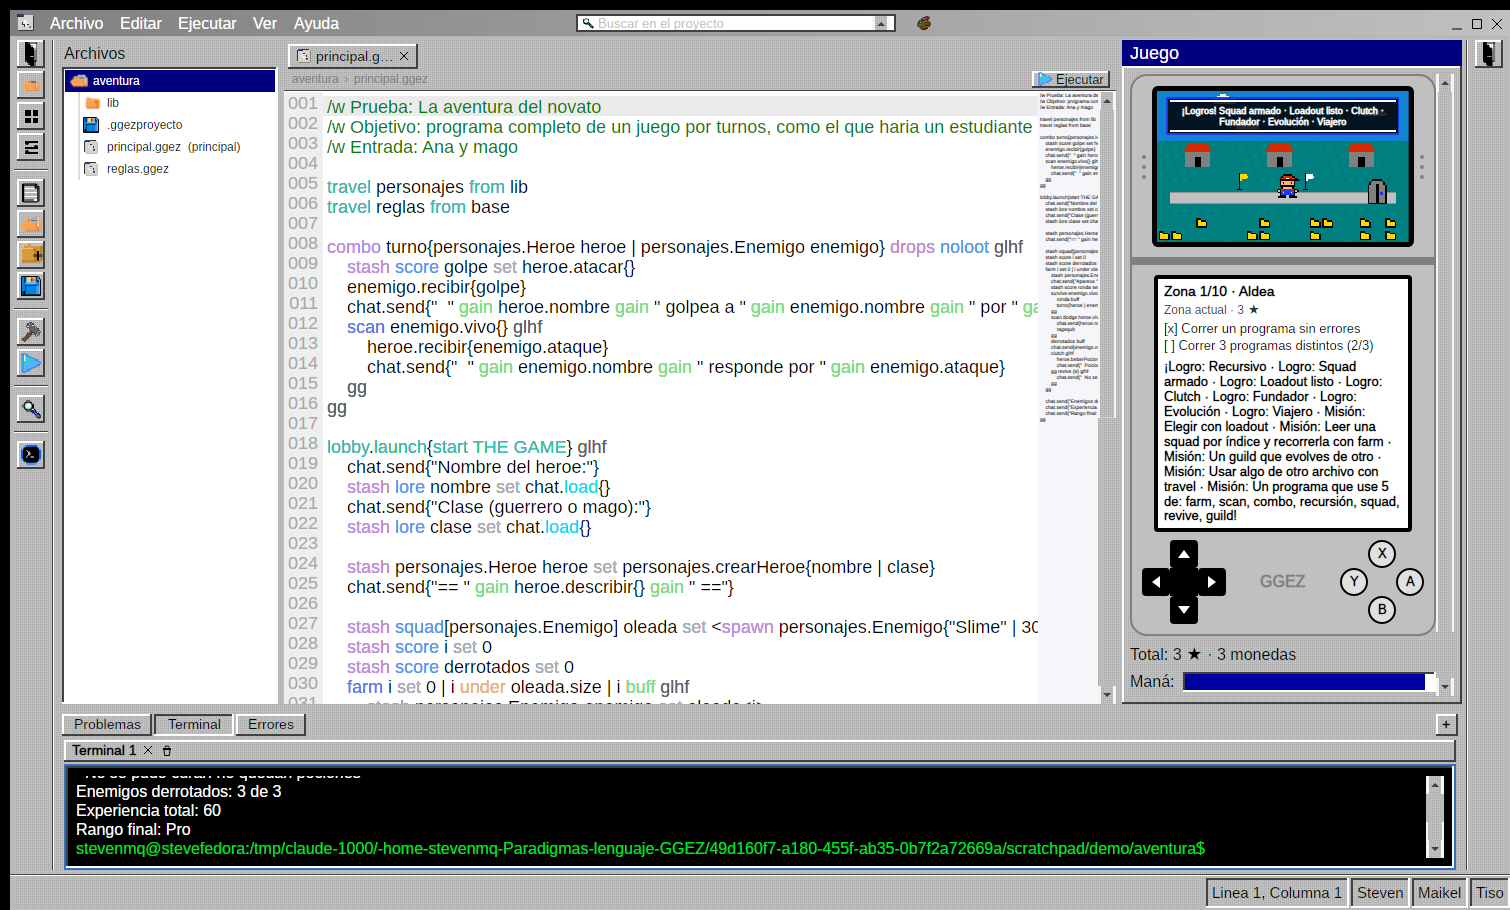
\includegraphics[width=0.92\textwidth]{img/ide_ejecucion.png}
\caption{Ejecución de un programa con entrada interactiva en la terminal integrada.}
\end{figure}

\subsection{Gestión de alcances}

Existe un entorno global con las funciones y tipos de cada archivo. Cada bloque (rama de un \kw{scan}, cuerpo de un ciclo, bloque de \kw{clutch}) crea un entorno hijo que se descarta al llegar a su \kw{gg}. Cada llamada a un \kw{combo} crea un entorno nuevo con sus parámetros, que no ve las variables de quien hizo la llamada. Dentro de un método, los nombres se buscan primero en las variables locales, después en los campos y métodos del objeto y por último en los \kw{combo} globales.

\subsection{Ejecución de importaciones}

Cuando el intérprete encuentra una llamada a un \kw{combo} importado (\kw{modulo.combo\{\}}), ejecuta el cuerpo de esa función con su propio entorno, aislado del archivo que la llamó, y devuelve el valor al punto de la llamada. Lo mismo ocurre con \kw{spawn modulo.Tipo\{\}}. Los archivos importados no ejecutan código propio: solo aportan declaraciones.

\subsection{Limitaciones de la ejecución}

\begin{itemize}
  \item \textbf{Maná.} Cada instrucción y cada vuelta de un ciclo gasta un punto. El programa empieza con 5\,000\,000; si se agota, termina con el error «sin mana». Así un ciclo infinito no congela el IDE. Este error no se puede atrapar con \kw{revive}.
  \item \textbf{Recursión.} La profundidad máxima es de 5000 llamadas anidadas; al superarla se produce un error que indica revisar el caso base.
  \item \textbf{Velocidad.} Un intérprete que recorre el árbol es más lento que un lenguaje compilado a código nativo, lo cual es aceptable para el propósito educativo del lenguaje.
\end{itemize}

\newpage
% ================================================================ 15
\section{Manejo de errores}
\label{sec:errores}

El sistema de manejo de errores es uno de los componentes centrales de \ggez, porque es lo primero que encuentra un principiante cuando algo sale mal. Esta sección documenta las categorías de errores, el formato de los mensajes y el comportamiento del aplicativo.

\subsection{Categorías de errores}

\begin{longtable}{|p{3cm}|p{4.4cm}|p{7cm}|}\hline
\cab\textbf{Categoría} & \textbf{Momento de detección} & \textbf{Ejemplos típicos} \\\hline\endhead
Léxicos & Análisis léxico (fase 1) & Caracteres no reconocidos, cadenas sin cerrar, nombres con tilde \\\hline
Sintácticos & Análisis sintáctico (fase 2) & Bloques sin \kw{gg}, \kw{combo} sin \kw{drops}, punto de entrada mal escrito, falta un valor \\\hline
De importación & Resolución de importaciones (fase 3) y llamadas a lo importado (fase 4) & Archivo o función inexistente, módulo duplicado, importación circular, argumentos incorrectos en una llamada importada \\\hline
Semánticos & Análisis semántico (fase 4) & Variable no declarada, tipos incompatibles, cantidad de argumentos, redeclaración, sin punto de entrada \\\hline
En ejecución & Interpretación del programa & División entre cero, índice fuera de rango, objeto \kw{afk}, \kw{wipe} no atrapado, sin maná, recursión excesiva \\\hline
De proyecto & En el IDE, antes de compilar & La pestaña enfocada no es un \kw{.ggez} y no hay archivo principal, o este fue borrado \\\hline
\end{longtable}

\subsection{Formato estándar de los mensajes}

Cada mensaje de error incluye: (1) el archivo, (2) la línea, (3) la columna, (4) el tipo de error, (5) una descripción del problema y (6) una posible causa. Se escribe en dos líneas:

\begin{lstlisting}[language={}]
principal.ggez:7:25: error semantico: 'escudo' no esta declarada
    posible causa: Declarela con stash antes de usarla, o revise si
    escribio mal el nombre o si quedo en otro bloque.
\end{lstlisting}

Para encontrar la posible causa, el traductor busca en el mensaje fragmentos conocidos (por ejemplo «no esta declarada» o «se obtuvo») y, si ninguno coincide, usa una sugerencia general según el tipo de error. Los mensajes evitan tildes para que se vean bien en cualquier consola.

En el IDE, la pestaña Problemas presenta cada error con su ícono, el archivo y la línea, la descripción y, debajo, la posible causa en gris.

\begin{figure}[H]
\centering
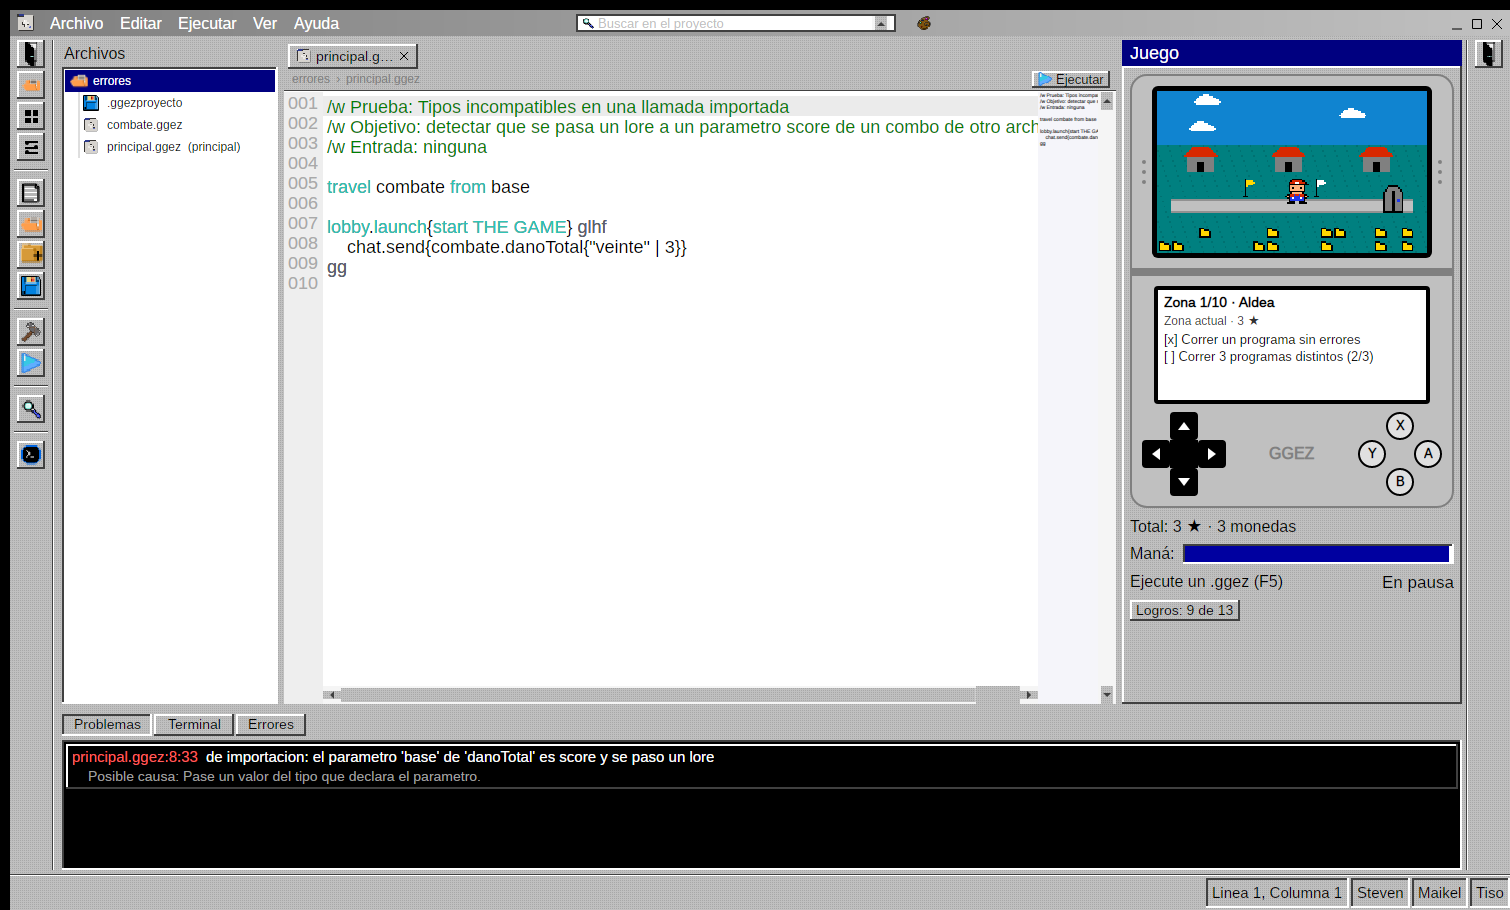
\includegraphics[width=0.92\textwidth]{img/problemas_error.png}
\caption{Pestaña Problemas con un error y su posible causa.}
\end{figure}

\subsection{Filosofía de retroalimentación}

Los mensajes de \ggez\ siguen cuatro principios: (1) \textbf{lenguaje claro}, en español y sin jerga innecesaria; (2) \textbf{ubicación precisa}, con archivo, línea y columna; (3) \textbf{orientación a la solución}, diciendo qué revisar y no solo qué falló; y (4) \textbf{un error a la vez}, para no abrumar.

\subsection{Comportamiento del aplicativo}

Un programa con errores de compilación no se ejecuta. Los errores en ejecución detienen el programa en el punto donde ocurren, salvo que se atrapen con \kw{clutch}/\kw{revive}. En ambos casos la terminal muestra el error en rojo y la pestaña Problemas lo lista; un clic sobre el problema abre el archivo y lleva el cursor a la línea. La pestaña Errores (menú Ejecutar, «Ver errores») conserva los mensajes del IDE. Cada vez que se compila o ejecuta, la pestaña Problemas se limpia y muestra solo el estado actual.

\subsection{Advertencias}

Cuando el programa compila sin errores, el compilador revisa además tres situaciones que no impiden ejecutar pero suelen indicar un descuido:

\begin{longtable}{|p{4cm}|p{10.4cm}|}\hline
\cab\textbf{Advertencia} & \textbf{Cuándo se reporta} \\\hline\endhead
Variable sin usar & Una variable declarada cuyo valor nunca se lee. Asignarle un valor no cuenta como leerla. \\\hline
\kw{combo} sin usar & Un \kw{combo} del archivo principal que nunca se llama; las llamadas a sí mismo no cuentan. Los archivos importados no se revisan, porque pueden tener funciones que el programa no necesita. \\\hline
Código que nunca se ejecuta & Instrucciones escritas después de un \kw{reward}, \kw{ragequit}, \kw{respawn} o \kw{wipe} en el mismo bloque. \\\hline
\end{longtable}

Las advertencias usan el mismo formato que los errores, con el tipo \kw{advertencia}, y el IDE las muestra en amarillo.

\begin{lstlisting}[language={}]
principal.ggez:6:5: advertencia: la variable 'oro' se declaro pero su valor nunca se usa
\end{lstlisting}

\begin{figure}[H]
\centering
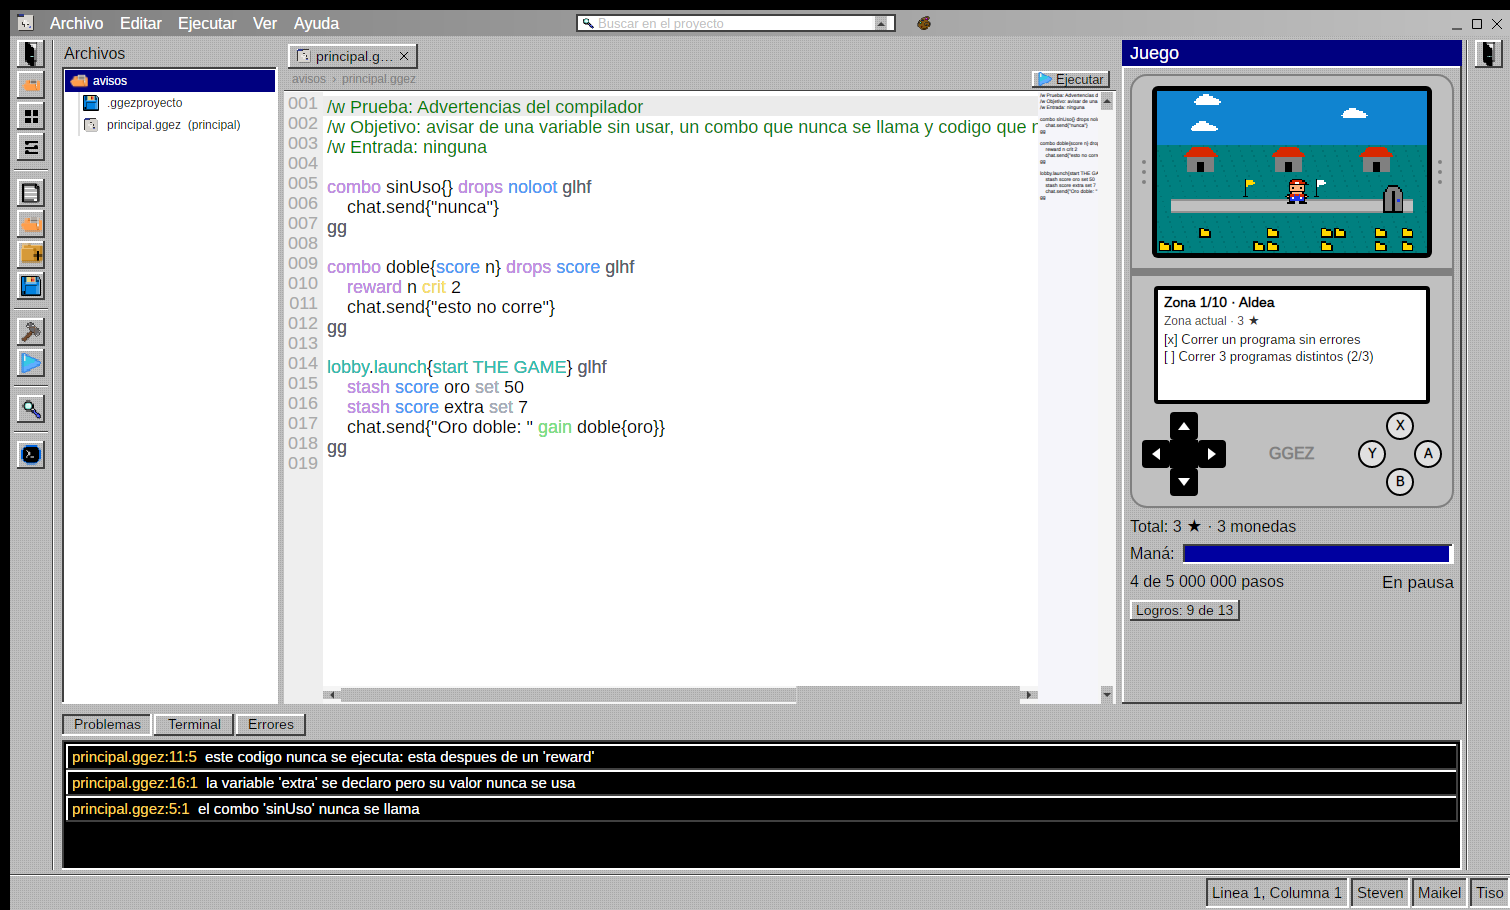
\includegraphics[width=0.92\textwidth]{img/advertencias.png}
\caption{Advertencias en amarillo en la terminal y en la pestaña Problemas.}
\end{figure}

\newpage
% ================================================================ 16
\section{Innovación}
\label{sec:innovacion}

La característica de innovación de \ggez\ es que \textbf{el entorno de desarrollo es en sí mismo un juego}, cuyo progreso depende de que el código del estudiante funcione de verdad. Se complementa con una terminal real con asistente de inteligencia artificial y un sistema de extensiones. Esta sección describe su funcionamiento, cómo se integra con el traductor y por qué se eligió.

\subsection{Descripción funcional}

El IDE tiene un panel de juego, a la derecha del editor, que muestra el maná, el mapa del mundo, el nivel actual, las monedas, las pistas y los logros. Cada vez que el estudiante ejecuta un programa, el traductor informa al IDE cuánto maná gastó, qué construcciones del lenguaje se ejecutaron y si obtuvo algún logro; el IDE actualiza el panel con esa información. Nada se gana con solo escribir código: solo cuenta lo que se ejecutó sin errores.

\subsection{Componentes}

\textbf{Maná.} Cada instrucción y cada vuelta de ciclo gasta un punto de maná, y la barra muestra cuánto gastó el programa. Además de impedir que un ciclo infinito congele el IDE, hace visible el costo de un algoritmo: un programa más eficiente gasta menos.

\textbf{Mundo y misiones.} Un mapa con diez zonas en orden: Aldea, Pradera, Bosque de los ciclos, Río, Cueva, Torre, Mercado, Castillo, Gremio y Guarida del jefe. Cada zona tiene misiones que se cumplen ejecutando programas que usen ciertas construcciones (por ejemplo, un programa con \kw{farm}, \kw{survive} y \kw{grind}, o uno con un \kw{guild} que \kw{evolves} de otro). Al completar las misiones de una zona se abre la siguiente.

\begin{figure}[H]
\centering
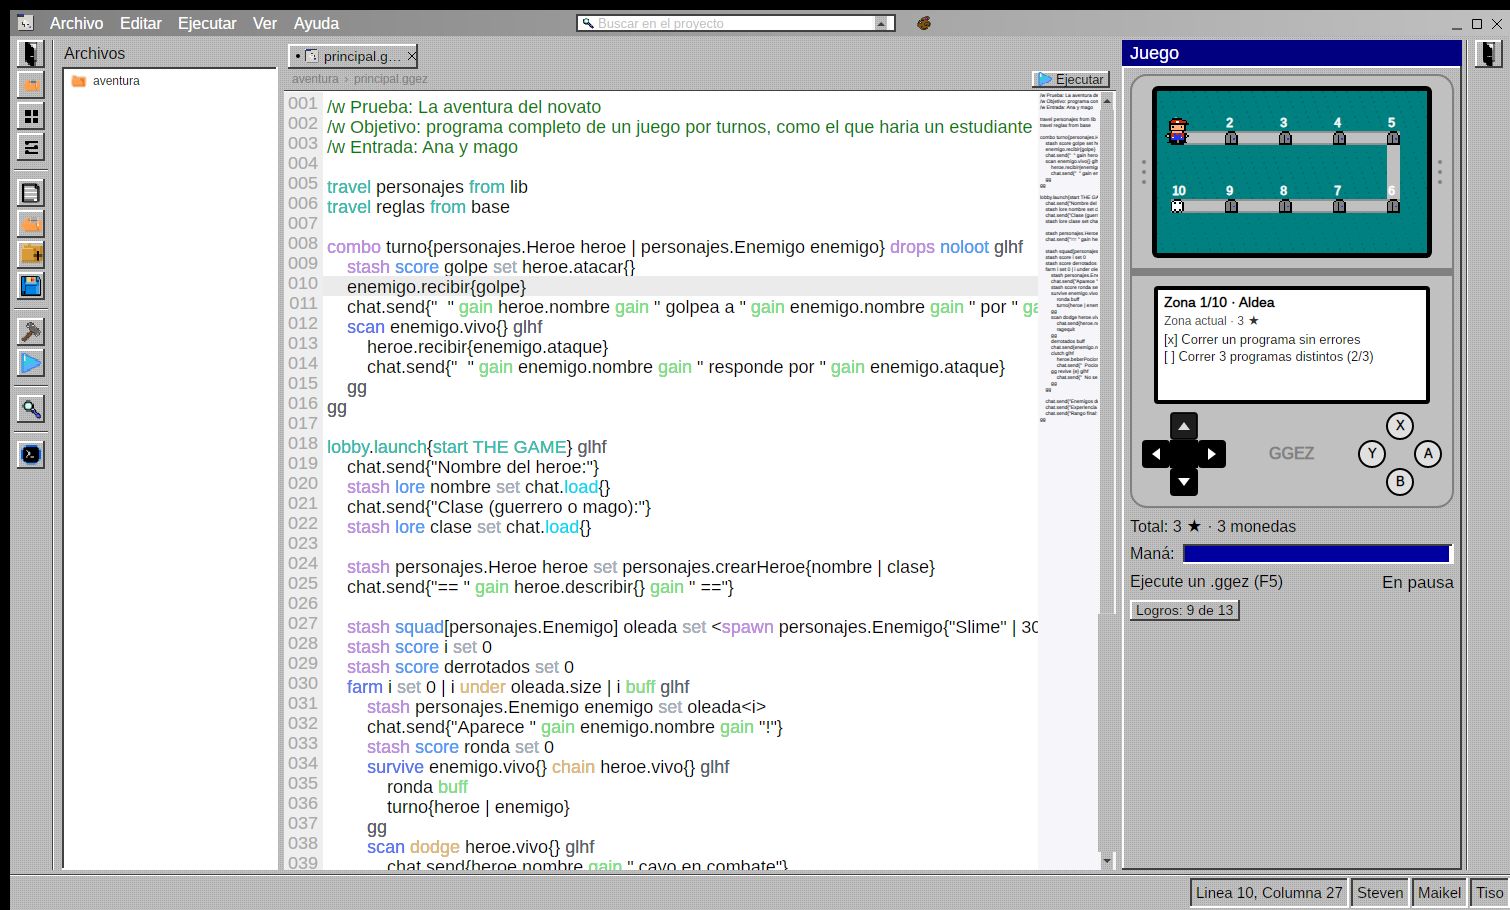
\includegraphics[width=0.8\textwidth]{img/mapa.png}
\caption{Mapa del mundo con la zona actual y sus misiones.}
\end{figure}

\textbf{Niveles y estrellas.} Una carpeta con un archivo \kw{nivel.json} define un reto: título, pruebas (una llamada o una entrada, con su salida esperada), pistas y una meta de pasos. Al ejecutar, el traductor corre las pruebas y el IDE otorga hasta tres estrellas: una por pasar todas las pruebas, otra por lograrlo al primer intento y otra por no superar la meta de pasos. Cualquier docente puede crear niveles nuevos con un archivo de texto, sin tocar el código del IDE.

\begin{lstlisting}[language={}]
{
  "titulo": "Suma de Gauss",
  "meta_pasos": 5,
  "pistas": ["Con un farm de 1 a n y boost se pasan las pruebas", "..."],
  "pruebas": [
    { "llamada": "sumarHasta{10}", "salida": "55" },
    { "llamada": "sumarHasta{0}",  "salida": "0" }
  ]
}
\end{lstlisting}

\textbf{Monedas y pistas.} Cada estrella ganada da una moneda, y cada pista de un nivel cuesta una. El estudiante decide si pide ayuda o lo intenta solo.

\textbf{Logros.} Trece logros reconocen hitos de aprendizaje: correr el primer programa sin errores, declarar un \kw{combo}, escribir una recursión, usar \kw{squad}, usar \kw{loadout}, usar los tres ciclos en un programa, atrapar un error, declarar un \kw{guild}, usar herencia, importar un archivo, quedarse sin maná, ganar tres estrellas en un nivel y comprar una pista. Al obtener uno, el IDE muestra una notificación.

\textbf{Temas desbloqueables.} Las estrellas desbloquean temas visuales para el editor (con 6, 15 y 25 estrellas), además de un modo oscuro disponible desde el inicio.

\textbf{Terminal real con asistente de inteligencia artificial.} El segmento de salida admite hasta cuatro terminales en columnas, con comandos propios (\kw{cd}, \kw{clear}, \kw{exit}, \kw{help}). Al instalar la extensión de Claude, las terminales pasan a ser terminales reales del sistema operativo, capaces de correr cualquier programa interactivo, entre ellos el asistente \kw{claude}. Así el estudiante puede pedir, dentro del mismo IDE, que le expliquen un error o un concepto.

\textbf{Sistema de extensiones.} Desde la vista de extensiones se instalan y desinstalan complementos: sangría de colores, resaltado de espacios al final de la línea, resaltado de \kw{TODO}, colores por nivel de bloques, modo oscuro, bloques al estilo Pac-Man, la terminal de Claude y los temas desbloqueables.

\begin{figure}[H]
\centering
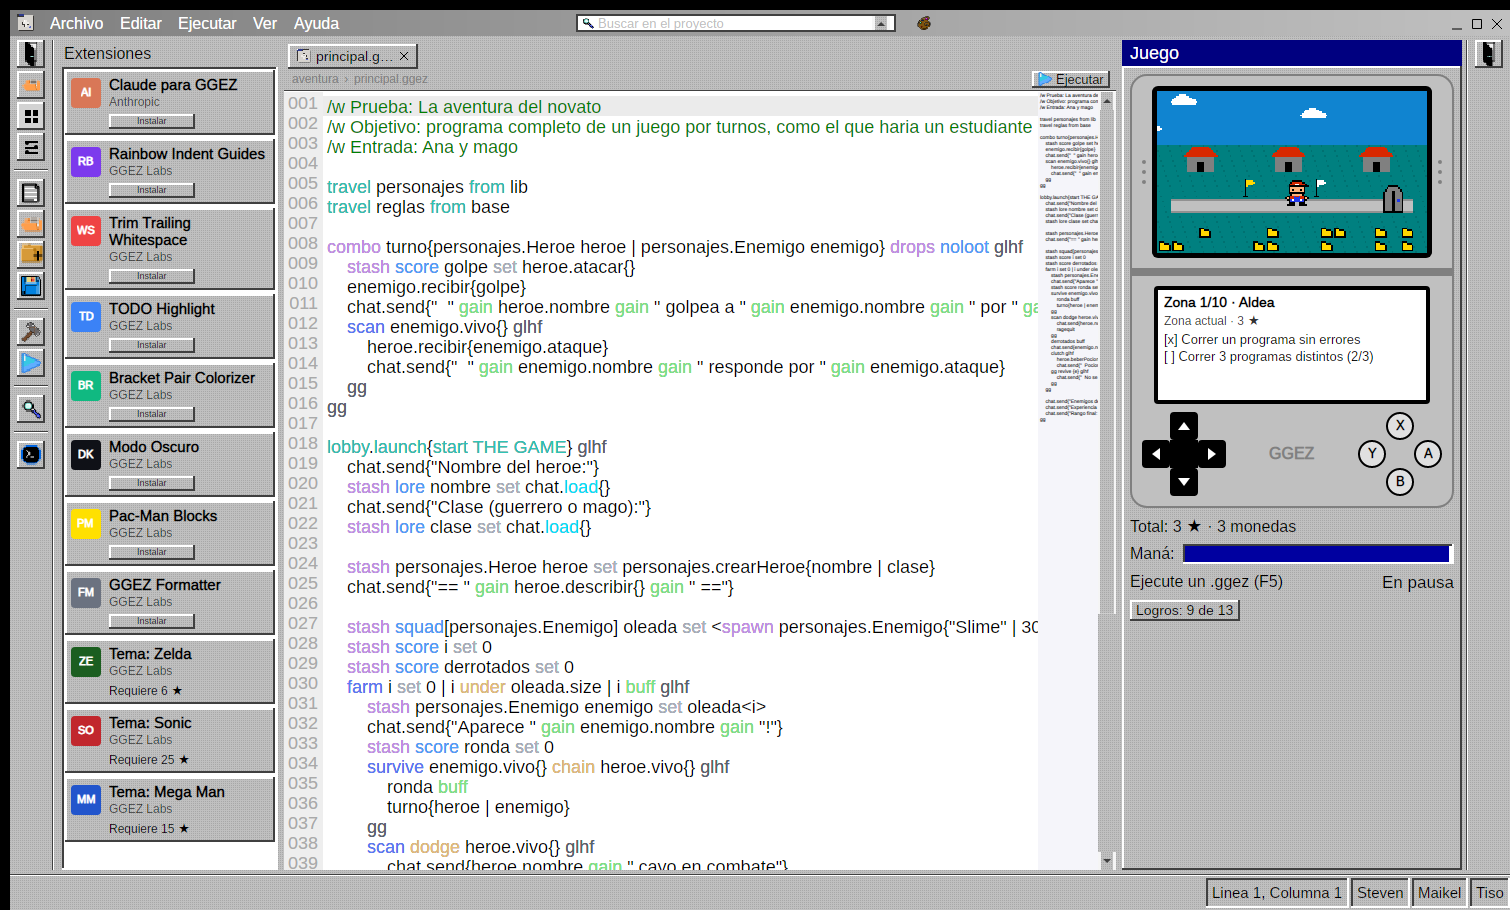
\includegraphics[width=0.92\textwidth]{img/extensiones.png}
\caption{Vista de extensiones.}
\end{figure}

\subsection{Funcionamiento técnico}

El IDE ejecuta el traductor con la opción \kw{--eventos}. Al terminar el programa, el traductor escribe en la salida líneas que empiezan con \kw{@ggez}, que el IDE no muestra en la terminal sino que envía al panel de juego:

\begin{longtable}{|p{5.4cm}|p{9cm}|}\hline
\cab\textbf{Evento} & \textbf{Significado} \\\hline\endhead
\kw{@ggez pasos <usados> <limite>} & Maná gastado y maná disponible. \\\hline
\kw{@ggez logro <id>} & El programa cumplió las condiciones de un logro. \\\hline
\kw{@ggez programa <huella> <usos>} & Huella del programa y construcciones que se ejecutaron (ciclos, recursión, clases, importaciones...), para avanzar las misiones. \\\hline
\kw{@ggez nivel <pasadas> <total> <pasos> <meta> <titulo>} & Resultado de las pruebas de un nivel, para calcular las estrellas. \\\hline
\end{longtable}

Las construcciones usadas se registran durante la ejecución, no al leer el código: un \kw{farm} que nunca dio una vuelta no cuenta. La huella identifica el programa, de modo que una misión que pide varios programas distintos no se cumple ejecutando el mismo dos veces. El progreso (estrellas, monedas, logros, misiones y récords de cada nivel) se guarda en el archivo \kw{progreso.json} de la carpeta de configuración del usuario.

\subsection{Validaciones e integración}

\begin{itemize}
  \item El archivo \kw{nivel.json} puede venir de otra persona, por lo que el traductor revisa su forma antes de usarlo (título de texto, meta de pasos entera y positiva, al menos una prueba con su salida, llamadas de una sola línea) y reporta un error claro si algo está mal.
  \item Un evento con un identificador que el IDE no conoce se ignora.
  \item Solo se puede comprar una pista si hay monedas suficientes y quedan pistas en el nivel.
  \item La gamificación no requiere configuración: funciona desde la primera ejecución y no interfiere con el programa, cuya salida se ve completa en la terminal.
\end{itemize}

\subsection{Justificación}

La elección de esta característica responde a tres consideraciones. Primero, atiende directamente el problema planteado: el estudiante de primer ingreso conoce los videojuegos y su sistema de progreso, y el IDE usa ese mismo lenguaje para mostrarle que está avanzando. Segundo, está ligada al aprendizaje real, porque solo avanza con código que se ejecuta y premia construcciones concretas del lenguaje, por lo que no es un adorno separado de la programación. Tercero, es demostrable durante la presentación: basta ejecutar un programa para ver cómo cambia el maná, se cumple una misión o aparece un logro.

\newpage
% ================================================================ 17
\section{Arquitectura del aplicativo}

El aplicativo tiene dos componentes que se comunican mediante procesos: el \textbf{IDE}, escrito en C\# con Avalonia, y el \textbf{traductor}, escrito en Python. Esta sección describe las tecnologías utilizadas, la organización en capas y los módulos del código fuente.

\subsection{Tecnologías utilizadas}

\begin{itemize}
  \item \textbf{C\# y .NET.} Lenguaje y plataforma del IDE.
  \item \textbf{Avalonia.} Biblioteca de interfaz gráfica multiplataforma que permite que el mismo IDE funcione en Linux y Windows.
  \item \textbf{CommunityToolkit.Mvvm.} Implementa el patrón Modelo-Vista-VistaModelo con propiedades observables y comandos.
  \item \textbf{RoyalTerminal.} Control de terminal que usa la extensión de Claude para ofrecer terminales reales.
  \item \textbf{Python 3.} Lenguaje del traductor, sin bibliotecas externas.
  \item \textbf{Python portátil (python-build-standalone).} Intérprete de Python que se incrusta en el ejecutable para que el usuario no tenga que instalarlo.
  \item \textbf{Nix.} El repositorio incluye un \kw{flake.nix} para preparar el entorno de desarrollo.
  \item \textbf{Git y GitHub.} Control de versiones y trabajo en equipo.
\end{itemize}

\subsection{Organización en capas}

\textbf{Capa de presentación (IDE).} Contiene todo lo visual: ventana principal, menús, árbol de archivos, editor, terminales, pestañas de errores y problemas, panel de juego, ayuda, extensiones y ajustes. Sigue el patrón MVVM: las vistas (\kw{.axaml}) solo muestran datos y los modelos de vista (\kw{ViewModels}) contienen la lógica de la interfaz.

\textbf{Frontera de integración.} El IDE y el traductor solo se comunican por texto: el IDE lanza \kw{ggezc} como un proceso, le pasa la entrada del usuario y lee su salida. Los errores tienen un formato fijo (\kw{archivo:linea:columna: tipo: mensaje}) que el IDE interpreta con una expresión regular, y los eventos del juego empiezan con \kw{@ggez}. Gracias a esto, el traductor puede usarse y probarse sin el IDE.

\textbf{Capa de lógica del lenguaje (traductor).} Contiene el compilador, el intérprete, las pruebas de niveles y los eventos del juego. No depende de la interfaz gráfica.

\textbf{Capa de servicios.} En el IDE, componentes de apoyo: diálogos, configuración, persistencia de la sesión y de las extensiones, temas, progreso del juego, procesos de las terminales e instalación del traductor incrustado.

\subsection{Estructura de módulos}

\begin{lstlisting}[language={}]
ParadigmasLenguajePropio/src/ParadigmasLenguajePropio/   (IDE)
    Views/          ventana, menu, barra de estado, explorador, extensiones,
                    ajustes, editor, terminal, panel de juego
    ViewModels/     logica de cada vista (abrir, guardar, ejecutar, errores)
    Models/         archivos del arbol, problemas, logros, mundo, ayuda
    Services/       dialogos, sesion, temas, progreso, terminales, instalacion
    Controls/       editor (coloreado, autocompletado, minimapa), arbol
    Themes/, Assets/   estilos, fuentes e iconos
Traductor/                                                 (traductor)
    ggezc.py        punto de entrada de la linea de comandos
    GRAMATICA.md    gramatica formal
    src/ggez/
        cli.py          comandos run, compile, check, tokens
        tokens.py       palabras reservadas
        lexer.py        analisis lexico
        sintactico.py   analisis sintactico
        arbol.py        nodos del arbol sintactico
        cargador.py     importaciones con travel
        semantico.py    analisis semantico y advertencias
        evaluador.py    interprete
        errores.py      formato de errores y posible causa
        nivel.py        pruebas de nivel.json
        logros.py       eventos del modo de juego
    pruebas/        casos de la seccion 18 y correr.py
    ejemplos/       programas de ejemplo
publicar.sh         genera el ejecutable unico
\end{lstlisting}

\subsection{Flujo de una operación típica}

Al presionar Compilar (\kw{F6}), el IDE guarda todos los archivos, limpia la pestaña Problemas, toma el archivo \kw{.ggez} enfocado (o el principal, si no hay uno) y lanza \kw{ggezc compile} en una terminal integrada. El traductor ejecuta las cuatro fases de la sección 13 y escribe «Compilacion exitosa» con sus advertencias, o un único error. El IDE lee la salida de errores línea por línea, colorea cada línea según su tipo y llena la pestaña Problemas. Al ejecutar (\kw{F5}) el flujo es el mismo con \kw{ggezc run --eventos}: la salida del programa aparece en la terminal, la entrada del usuario se envía al proceso y, al terminar, los eventos \kw{@ggez} actualizan el panel de juego.

\subsection{Distribución}

El entregable es un ejecutable único por sistema operativo, generado con el script \kw{publicar.sh} de la raíz del repositorio (\kw{./publicar.sh linux}, \kw{windows} o \kw{todo}). El script publica el IDE como un solo archivo y le incrusta un Python portátil y el traductor; la primera vez que se abre, el IDE los despliega en la carpeta de datos del usuario. Así el estudiante no necesita instalar .NET ni Python.

\subsection{Consideraciones de diseño}

La separación entre IDE y traductor fue la decisión principal de la arquitectura: permitió que los integrantes trabajaran en paralelo, que el traductor se probara de forma automática sin interfaz y que el formato de errores fuera un contrato simple entre ambos. El patrón MVVM mantiene la interfaz separada de su lógica, y concentrar las palabras reservadas en un solo archivo hace que el lenguaje pueda ajustarse sin tocar el resto del traductor.

\newpage

% ================================================================ 18
\section{Pruebas}
\label{sec:pruebas}

Esta sección documenta la batería de pruebas realizadas sobre \ggez\ para verificar su funcionamiento. Las pruebas se organizan según las categorías establecidas por el enunciado del proyecto, y cada una indica su objetivo, entrada, resultado esperado, resultado obtenido y estado (aprobada o reprobada).

Cada caso es un proyecto \ggez\ real guardado en el repositorio, dentro de una carpeta por categoría en \kw{Traductor/pruebas/}: \kw{1\_validos/}, \kw{2\_sintacticos/}, \kw{3\_semanticos/}, \kw{4\_importaciones/}, \kw{5\_circular/}, \kw{6\_completa/} y \kw{7\_advertencias/}. Cada caso tiene su \kw{principal.ggez} (con una cabecera de comentarios que documenta la prueba, su objetivo y su entrada), un archivo \kw{esperado.txt} con la salida esperada completa (salida estándar, salida de errores y código de salida) y, si el programa lee datos, un archivo \kw{entrada.txt}.

El script \kw{pruebas/correr.py} ejecuta cada caso con el traductor real y compara la salida obtenida con la esperada; se ejecuta con \kw{make test} desde la carpeta \kw{Traductor}. Las tablas de esta sección se generaron con ese mismo script (\kw{python pruebas/correr.py --latex}), por lo que el resultado obtenido corresponde a una ejecución real. Los números de línea de los mensajes corresponden al archivo del caso, incluida su cabecera de comentarios. Las 23 pruebas resultaron aprobadas.

\begin{longtable}{|p{7.4cm}|p{2.6cm}|p{2.6cm}|}\hline
\cab\textbf{Categoría} & \textbf{Casos} & \textbf{Aprobados} \\\hline\endhead
Programas válidos & 5 & 5 \\\hline
Errores sintácticos & 5 & 5 \\\hline
Errores semánticos & 5 & 5 \\\hline
Importaciones & 5 & 5 \\\hline
Importación circular & 1 & 1 \\\hline
Prueba completa relacionada con el problema & 1 & 1 \\\hline
Advertencias & 1 & 1 \\\hline
\textbf{Total} & \textbf{23} & \textbf{23} \\\hline
\end{longtable}

\subsection{Programas válidos}
\label{pr:1_validos}
Casos de la carpeta \texttt{pruebas/1\_validos/}.

\begin{tablaprueba}
1. Tipos simples y operaciones. Declarar los cinco tipos simples y una constante, y usar operaciones aritméticas, relacionales y lógicas & \texttt{1\_\allowbreak{}validos/\allowbreak{}01\_\allowbreak{}tipos\_\allowbreak{}y\_\allowbreak{}operaciones}. Entrada: ninguna & {\ttfamily\footnotesize Novato (rango B)\newline Vida tras 2 golpes: 70\newline Dano critico: 11.25\newline 17 split 5 = 3, 17 scrap 5 = 2\newline Sigue vivo: hit\newline Sin escudo: miss\newline Vida igual a 100: hit, distinta de 50: hit\newline [codigo de salida 0]} & Igual al esperado. \textbf{Aprobada} \\ \hline
2. Entrada de datos y condicionales. Leer datos con chat.load y decidir con scan, fallback y loadout & \texttt{1\_\allowbreak{}validos/\allowbreak{}02\_\allowbreak{}entrada\_\allowbreak{}y\_\allowbreak{}condicionales}. Entrada: Ana y mago & {\ttfamily\footnotesize Nombre del jugador:\newline Clase (guerrero, mago o arquero):\newline Bienvenido, Ana. Poder: 95\newline Rango: Pro\newline [codigo de salida 0]} & Igual al esperado. \textbf{Aprobada} \\ \hline
3. Ciclos. Usar farm (for), survive (while) y grind (do-while), con ragequit y respawn & \texttt{1\_\allowbreak{}validos/\allowbreak{}03\_\allowbreak{}ciclos}. Entrada: ninguna & {\ttfamily\footnotesize Monedas (1..6 sin el 3): 18\newline Quedan 3 enemigos\newline Quedan 2 enemigos\newline Quedan 1 enemigos\newline El grind corre al menos una vez\newline [codigo de salida 0]} & Igual al esperado. \textbf{Aprobada} \\ \hline
4. Funciones, recursión y squad. Combos con y sin retorno, parámetros, recursión directa y operaciones de squad & \texttt{1\_\allowbreak{}validos/\allowbreak{}04\_\allowbreak{}funciones\_\allowbreak{}y\_\allowbreak{}listas}. Entrada: ninguna & {\ttfamily\footnotesize 5! = 120\newline - Tanque\newline - Sanador\newline - Arquero\newline Ahora son 2, el primero es Curandero\newline [codigo de salida 0]} & Igual al esperado. \textbf{Aprobada} \\ \hline
5. Registros, clases, herencia y manejo de errores. Usar inventory, guild con evolves y clutch/revive/checkpoint & \texttt{1\_\allowbreak{}validos/\allowbreak{}05\_\allowbreak{}objetos\_\allowbreak{}y\_\allowbreak{}errores}. Entrada: ninguna & {\ttfamily\footnotesize Espada tiene poder 40\newline Conan: POR LA GLORIA!\newline Error atrapado en la linea 44: division entre cero\newline El checkpoint siempre corre\newline [codigo de salida 0]} & Igual al esperado. \textbf{Aprobada} \\ \hline
\end{tablaprueba}

\subsection{Errores sintácticos}
\label{pr:2_sintacticos}
Casos de la carpeta \texttt{pruebas/2\_sintacticos/}.

\begin{tablaprueba}
1. Bloque sin cerrar. Detectar un glhf al que le falta su gg & \texttt{2\_\allowbreak{}sintacticos/\allowbreak{}01\_\allowbreak{}bloque\_\allowbreak{}sin\_\allowbreak{}gg}. Entrada: ninguna & {\ttfamily\footnotesize principal.ggez:5:30: error sintactico: bloque sin cerrar: falta 'gg'\newline     posible causa: Cada glhf necesita su gg. Revise que no se haya borrado un gg al final de un bloque.\newline [codigo de salida 1]} & Igual al esperado. \textbf{Aprobada} \\ \hline
2. Combo sin drops. Detectar un combo que no declara su tipo de retorno con drops & \texttt{2\_\allowbreak{}sintacticos/\allowbreak{}02\_\allowbreak{}combo\_\allowbreak{}sin\_\allowbreak{}drops}. Entrada: ninguna & {\ttfamily\footnotesize principal.ggez:5:25: error sintactico: se esperaba 'drops' y se encontro 'glhf'\newline     posible causa: Revise el orden de las palabras en esta linea comparandolo con la sintaxis en Ayuda.\newline [codigo de salida 1]} & Igual al esperado. \textbf{Aprobada} \\ \hline
3. Punto de entrada mal escrito. Detectar que start THE GAME es texto fijo obligatorio & \texttt{2\_\allowbreak{}sintacticos/\allowbreak{}03\_\allowbreak{}punto\_\allowbreak{}de\_\allowbreak{}entrada\_\allowbreak{}mal\_\allowbreak{}escrito}. Entrada: ninguna & {\ttfamily\footnotesize principal.ggez:5:20: error sintactico: se esperaba 'THE' y se encontro 'GAME'\newline     posible causa: Revise el orden de las palabras en esta linea comparandolo con la sintaxis en Ayuda.\newline [codigo de salida 1]} & Igual al esperado. \textbf{Aprobada} \\ \hline
4. Condicional sin glhf. Detectar un scan cuya condición no va seguida de glhf & \texttt{2\_\allowbreak{}sintacticos/\allowbreak{}04\_\allowbreak{}scan\_\allowbreak{}sin\_\allowbreak{}glhf}. Entrada: ninguna & {\ttfamily\footnotesize principal.ggez:7:21: error sintactico: se esperaba 'glhf' y se encontro un salto de linea\newline     posible causa: Revise el orden de las palabras en esta linea comparandolo con la sintaxis en Ayuda.\newline [codigo de salida 1]} & Igual al esperado. \textbf{Aprobada} \\ \hline
5. Declaración sin valor. Detectar un set al que le falta la expresión & \texttt{2\_\allowbreak{}sintacticos/\allowbreak{}05\_\allowbreak{}falta\_\allowbreak{}valor}. Entrada: ninguna & {\ttfamily\footnotesize principal.ggez:6:25: error sintactico: se esperaba una expresion y se encontro un salto de linea\newline     posible causa: Revise el orden de las palabras en esta linea comparandolo con la sintaxis en Ayuda.\newline [codigo de salida 1]} & Igual al esperado. \textbf{Aprobada} \\ \hline
\end{tablaprueba}

\subsection{Errores semánticos}
\label{pr:3_semanticos}
Casos de la carpeta \texttt{pruebas/3\_semanticos/}.

\begin{tablaprueba}
1. Variable no declarada. Detectar el uso de una variable que nunca se declaró con stash & \texttt{3\_\allowbreak{}semanticos/\allowbreak{}01\_\allowbreak{}no\_\allowbreak{}declarada}. Entrada: ninguna & {\ttfamily\footnotesize principal.ggez:7:25: error semantico: 'escudo' no esta declarada\newline     posible causa: Declarela con stash antes de usarla, o revise si escribio mal el nombre o si quedo en otro bloque.\newline [codigo de salida 1]} & Igual al esperado. \textbf{Aprobada} \\ \hline
2. Tipos incompatibles. Detectar que se guarda un lore en una variable score & \texttt{3\_\allowbreak{}semanticos/\allowbreak{}02\_\allowbreak{}tipos\_\allowbreak{}incompatibles}. Entrada: ninguna & {\ttfamily\footnotesize principal.ggez:6:5: error semantico: se esperaba score y se obtuvo lore\newline     posible causa: Los tipos no coinciden: use un valor del tipo declarado (score, aim, lore, win, pixel...).\newline [codigo de salida 1]} & Igual al esperado. \textbf{Aprobada} \\ \hline
3. Cantidad de argumentos. Detectar una llamada con menos argumentos que parámetros & \texttt{3\_\allowbreak{}semanticos/\allowbreak{}03\_\allowbreak{}cantidad\_\allowbreak{}argumentos}. Entrada: ninguna & {\ttfamily\footnotesize principal.ggez:10:21: error semantico: el combo 'atacar' espera 2 argumento(s) y recibio 1\newline     posible causa: Revise la firma del combo: la cantidad de valores entre \{ \} debe ser igual a la de parametros.\newline [codigo de salida 1]} & Igual al esperado. \textbf{Aprobada} \\ \hline
4. Redeclaración. Detectar dos stash con el mismo nombre en el mismo bloque & \texttt{3\_\allowbreak{}semanticos/\allowbreak{}04\_\allowbreak{}redeclaracion}. Entrada: ninguna & {\ttfamily\footnotesize principal.ggez:7:5: error semantico: 'oro' ya fue declarada en este bloque\newline     posible causa: Para cambiar su valor use set sin stash.\newline [codigo de salida 1]} & Igual al esperado. \textbf{Aprobada} \\ \hline
5. Archivo principal sin punto de entrada. Detectar que el archivo principal no tiene lobby.launch & \texttt{3\_\allowbreak{}semanticos/\allowbreak{}05\_\allowbreak{}sin\_\allowbreak{}punto\_\allowbreak{}de\_\allowbreak{}entrada}. Entrada: ninguna & {\ttfamily\footnotesize principal.ggez:1:1: error semantico: el programa no tiene punto de entrada: falta lobby.launch\{start THE GAME\}\newline     posible causa: Agregue lobby.launch\{start THE GAME\} glhf ... gg en el archivo principal.\newline [codigo de salida 1]} & Igual al esperado. \textbf{Aprobada} \\ \hline
\end{tablaprueba}

\subsection{Pruebas de importaciones}
\label{pr:4_importaciones}
Casos de la carpeta \texttt{pruebas/4\_importaciones/}.

\begin{tablaprueba}
1. Importación válida. Usar combos y tipos de un archivo de la misma carpeta (base) y de una subcarpeta (lib) & \texttt{4\_\allowbreak{}importaciones/\allowbreak{}01\_\allowbreak{}importacion\_\allowbreak{}valida}. Entrada: ninguna & {\ttfamily\footnotesize Dano: 60\newline Pocion cuesta 25 monedas\newline [codigo de salida 0]} & Igual al esperado. \textbf{Aprobada} \\ \hline
2. Archivo importado inexistente. Detectar un travel a un archivo que no existe & \texttt{4\_\allowbreak{}importaciones/\allowbreak{}02\_\allowbreak{}archivo\_\allowbreak{}inexistente}. Entrada: ninguna & {\ttfamily\footnotesize principal.ggez:5:1: error de importacion: no existe inventario.ggez en la misma carpeta\newline     posible causa: Revise el nombre del archivo o tipo y la carpeta indicada en el from.\newline [codigo de salida 1]} & Igual al esperado. \textbf{Aprobada} \\ \hline
3. Combo inexistente en el módulo. Detectar la llamada a un combo que el archivo importado no define & \texttt{4\_\allowbreak{}importaciones/\allowbreak{}03\_\allowbreak{}combo\_\allowbreak{}inexistente}. Entrada: ninguna & {\ttfamily\footnotesize principal.ggez:8:22: error de importacion: el modulo combate no tiene 'curar'. Tiene: danoTotal\newline     posible causa: Revise el nombre: el mensaje lista lo que si existe.\newline [codigo de salida 1]} & Igual al esperado. \textbf{Aprobada} \\ \hline
4. Tipos incompatibles en una llamada importada. Detectar que se pasa un lore a un parámetro score de un combo de otro archivo & \texttt{4\_\allowbreak{}importaciones/\allowbreak{}04\_\allowbreak{}tipos\_\allowbreak{}en\_\allowbreak{}llamada\_\allowbreak{}importada}. Entrada: ninguna & {\ttfamily\footnotesize principal.ggez:8:33: error de importacion: el parametro 'base' de 'danoTotal' es score y se paso un lore\newline     posible causa: Pase un valor del tipo que declara el parametro.\newline [codigo de salida 1]} & Igual al esperado. \textbf{Aprobada} \\ \hline
5. Error dentro de un archivo importado. Detectar y ubicar un error que está en el archivo importado, no en el principal & \texttt{4\_\allowbreak{}importaciones/\allowbreak{}05\_\allowbreak{}error\_\allowbreak{}en\_\allowbreak{}importado}. Entrada: ninguna & {\ttfamily\footnotesize combate.ggez:2:22: error semantico: 'golpez' no esta declarada\newline     posible causa: Declarela con stash antes de usarla, o revise si escribio mal el nombre o si quedo en otro bloque.\newline [codigo de salida 1]} & Igual al esperado. \textbf{Aprobada} \\ \hline
\end{tablaprueba}

\subsection{Prueba de importación circular}
\label{pr:5_circular}
Casos de la carpeta \texttt{pruebas/5\_circular/}.

\begin{tablaprueba}
1. Importación circular. Detectar el ciclo mapa -> zona -> mapa & \texttt{5\_\allowbreak{}circular/\allowbreak{}01\_\allowbreak{}circular}. Entrada: ninguna & {\ttfamily\footnotesize zona.ggez:1:1: error de importacion: importacion en circulo: mapa.ggez -> zona.ggez -> mapa.ggez\newline     posible causa: Elimine uno de los travel del ciclo para que ningun archivo dependa de si mismo.\newline [codigo de salida 1]} & Igual al esperado. \textbf{Aprobada} \\ \hline
\end{tablaprueba}

\subsection{Prueba completa relacionada con el problema}
\label{pr:6_completa}
Casos de la carpeta \texttt{pruebas/6\_completa/}.

\begin{tablaprueba}
1. La aventura del novato. Programa completo de un juego por turnos, como el que haría un estudiante de primer ingreso: módulos, clases con herencia, squad, ciclos, condicionales, recursión, entrada de datos y manejo de errores & \texttt{6\_\allowbreak{}completa/\allowbreak{}01\_\allowbreak{}aventura\_\allowbreak{}del\_\allowbreak{}novato}. Entrada: Ana y mago & {\ttfamily\footnotesize Nombre del heroe:\newline Clase (guerrero o mago):\newline == Ana el mago (vida 80, ataque 30) ==\newline Aparece Slime!\newline   Ana golpea a Slime por 30\newline Slime derrotado en 1 ronda(s)\newline   Pocion: vida = 110\newline Aparece Goblin!\newline   Ana golpea a Goblin por 30\newline   Goblin responde por 7\newline   Ana golpea a Goblin por 30\newline Goblin derrotado en 2 ronda(s)\newline   Pocion: vida = 133\newline Aparece Dragon!\newline   Ana golpea a Dragon por 30\newline   Dragon responde por 12\newline   Ana golpea a Dragon por 30\newline   Dragon responde por 12\newline   Ana golpea a Dragon por 30\newline Dragon derrotado en 3 ronda(s)\newline   No se pudo curar: no quedan pociones\newline Enemigos derrotados: 3 de 3\newline Experiencia total: 60\newline Rango final: Pro\newline [codigo de salida 0]} & Igual al esperado. \textbf{Aprobada} \\ \hline
\end{tablaprueba}

\subsection{Advertencias}
\label{pr:7_advertencias}
Casos de la carpeta \texttt{pruebas/7\_advertencias/}.

\begin{tablaprueba}
1. Advertencias del compilador. Avisar de una variable sin usar, un combo que nunca se llama y código que nunca se ejecuta, sin impedir la ejecución & \texttt{7\_\allowbreak{}advertencias/\allowbreak{}01\_\allowbreak{}advertencias}. Entrada: ninguna & {\ttfamily\footnotesize Oro doble: 100\newline principal.ggez:11:5: advertencia: este codigo nunca se ejecuta: esta despues de un 'reward'\newline principal.ggez:16:1: advertencia: la variable 'extra' se declaro pero su valor nunca se usa\newline principal.ggez:5:1: advertencia: el combo 'sinUso' nunca se llama\newline [codigo de salida 0]} & Igual al esperado. \textbf{Aprobada} \\ \hline
\end{tablaprueba}


La prueba completa (\kw{6\_completa/01\_aventura\_del\_novato}) es un pequeño juego de rol por turnos, el tipo de programa que un estudiante de primer ingreso querría escribir. Está dividida en tres archivos: \kw{lib/personajes.ggez} con un \kw{inventory} y los \kw{guild} de los personajes (con herencia y polimorfismo); \kw{reglas.ggez} con los \kw{combo} de las reglas de daño (con recursión y manejo de errores); y \kw{principal.ggez}, que pide el nombre y la clase del jugador con \kw{chat.load}, arma el equipo en un \kw{squad} y simula el combate con ciclos y condicionales.

Además de estas pruebas automáticas, el entorno de desarrollo se verificó manualmente: crear y abrir un proyecto, compilar con \kw{F6}, ejecutar con \kw{F5} con entrada interactiva, ver un error en Problemas con su posible causa y saltar a la línea con un clic, ver advertencias y obtener logros y avanzar misiones. Las capturas de este documento se tomaron durante esas verificaciones.

\newpage
% ================================================================ 19
\section{Contribuciones de los integrantes}

Esta sección documenta la contribución de cada integrante al desarrollo del proyecto, según el historial del repositorio en GitHub (\url{https://github.com/VstevenMata/Paradigmas_lenguaje_GGEZ}). Se organiza por integrante e indica los componentes desarrollados y las pruebas realizadas.

{\small
\begin{longtable}{|p{2.6cm}|p{7.6cm}|p{4.2cm}|}\hline
\cab\textbf{Integrante} & \textbf{Componentes desarrollados} & \textbf{Pruebas realizadas} \\\hline\endhead
Steven Mata Quirós &
Entorno de desarrollo: ventana principal, menús, explorador de archivos, editor con pestañas y paneles divididos, coloreado, autocompletado, minimapa, búsqueda, terminales integradas, pestañas de errores y problemas, extensiones y temas, terminal de Claude, persistencia de la sesión y ayuda del lenguaje. Modo de juego: maná, niveles, estrellas, monedas, pistas, logros y mundo con misiones. Botones de compilar y ejecutar, archivo principal del proyecto, posible causa de los errores, advertencias, ejecutable único con \kw{publicar.sh} y documentación. &
Batería de pruebas de la sección 18 (\kw{pruebas/} y \kw{correr.py}) y verificación manual del entorno de desarrollo. \\\hline
Maikel Segura Quirós &
Primera versión de la terminal integrada. En el traductor: clases, herencia y manejo de errores (\kw{clutch}/\kw{revive}), e importaciones con \kw{travel} (\kw{cargador.py}). Extensión de colores e íconos. &
Programas de ejemplo de clases, errores e importaciones. \\\hline
Angel Ureña Naranjo &
Gramática formal (\kw{GRAMATICA.md}). Analizador léxico, sintáctico y semántico, e intérprete: control de flujo, funciones, vectores y registros. Conexión del botón de ejecutar del IDE con el traductor. &
Programas de ejemplo del lenguaje (\kw{Traductor/ejemplos/}). \\\hline
\end{longtable}
}

El diseño del lenguaje (vocabulario, tipos y reglas) se discutió y decidió en equipo; las decisiones quedaron registradas en \kw{Traductor/GRAMATICA.md}.

\newpage
% ================================================================ 20
\section{Conclusiones}

Esta sección presenta las conclusiones del proyecto, respondiendo a los objetivos planteados en la sección 5 y reflexionando sobre las decisiones de diseño, lo que se ajustaría en una segunda iteración y las limitaciones encontradas.

Los objetivos de la sección 5.2 se cumplieron. Definimos formalmente el lenguaje, con 71 palabras reservadas tomadas de los videojuegos, cinco tipos simples, dos compuestos, clases y reglas precisas de alcance y de importación. El compilador realiza las cuatro fases descritas en la sección 13, incluida la detección de importaciones circulares, y el intérprete ejecuta el árbol sintáctico sin recurrir a \kw{eval} ni \kw{exec}. El entorno de desarrollo propio integra editor, árbol de archivos, terminal, pestañas de errores y problemas, consulta del lenguaje y botones de compilar y ejecutar, y la gamificación ligada a la ejecución cumple el papel de innovación. Como evidencia, las 23 pruebas de la sección 18 se aprueban y el aplicativo se genera como un ejecutable único.

Entre las decisiones de diseño, consideramos acertadas las que acercan el lenguaje al estudiante sin alejarlo de los lenguajes profesionales: el vocabulario de videojuegos sobre una estructura igual a la de Java, los bloques \kw{glhf}/\kw{gg} en lugar de la indentación significativa, los operadores escritos con palabras (que eliminan la confusión entre \kw{=} y \kw{==}), el tipado estático que detecta errores antes de ejecutar, y los mensajes de error con posible causa. Separar el traductor del IDE y comunicarlos con un formato de texto simple permitió trabajar en paralelo y probar el traductor de forma automática.

En una segunda iteración, acordaríamos desde el inicio el formato de los errores y la batería de pruebas, que en este proyecto se completaron al final, y probaríamos antes el ejecutable en Windows. También implementaríamos lo que quedó reservado (interfaces, pilas, colas y la biblioteca \kw{arsenal}), la conversión de texto a número, el formateador automático y un depurador paso a paso.

Reconocemos varias limitaciones. \ggez\ no se ha evaluado con estudiantes de primer ingreso, por lo que su efecto sobre la motivación se basa en la observación del equipo y no en una medición. El ejecutable de Windows no se ha probado en un equipo real, el intérprete es lento para programas grandes y la recursión se limita a 5000 llamadas anidadas.

\newpage
% ================================================================ 21
\section{Referencias}

El proyecto no utilizó fuentes bibliográficas externas. A continuación se listan los documentos del curso y del equipo que guiaron el trabajo, y las herramientas de software utilizadas.

\begingroup
\setlength{\parindent}{-1.27cm}
\setlength{\leftskip}{1.27cm}

\textbf{Documentos}

Universidad Nacional. (2026). \emph{Descripción del Proyecto 2026} [Enunciado del proyecto del curso Paradigmas de Programación]. Sede Regional Brunca.

\emph{Problemas de traducción de lenguajes}. (s.f.). [Material del curso Paradigmas de Programación, Universidad Nacional].

Mata Quirós, S., Segura Quirós, M. y Ureña Naranjo, A. (2026). \emph{Propuesta de Lenguaje GGEZ} [Documento interno del equipo].

Mata Quirós, S., Segura Quirós, M. y Ureña Naranjo, A. (2026). \emph{Gramática formal de GGEZ} [Archivo \kw{Traductor/GRAMATICA.md} del repositorio del proyecto].

\textbf{Herramientas de software}

AvaloniaUI. (s.f.). \emph{Avalonia} (versión 12.1.1) [Software]. \url{https://avaloniaui.net}

Microsoft. (s.f.). \emph{.NET} [Software]. \url{https://dotnet.microsoft.com}

Microsoft. (s.f.). \emph{CommunityToolkit.Mvvm} (versión 8.4.2) [Software]. \url{https://github.com/CommunityToolkit/dotnet}

RoyalApps. (s.f.). \emph{RoyalApps.RoyalTerminal.Avalonia} (versión 0.5.2) [Software]. \url{https://www.nuget.org/packages/RoyalApps.RoyalTerminal.Avalonia}

Python Software Foundation. (2024). \emph{Python} (versión 3.12) [Software]. \url{https://www.python.org}

Astral. (2024). \emph{python-build-standalone} [Software]. \url{https://github.com/astral-sh/python-build-standalone}

\endgroup

\newpage
% ================================================================ 22
\section{Anexos}

\subsection{Manual de usuario de GGEZ}

\newcommand{\manualseccion}[1]{\subsubsection*{#1}}
% Manual de usuario: lo usan documentacion.tex (anexo) y manual_usuario.tex (aparte)
\manualseccion{Instalación}

\ggez\ se entrega como un único archivo ejecutable, generado con \kw{publicar.sh}. No requiere instalar .NET ni Python.

\begin{itemize}
  \item \textbf{Linux}: dar permiso de ejecución y abrirlo: \kw{chmod +x GGEZ} y luego \kw{./GGEZ}.
  \item \textbf{Windows}: abrir \kw{GGEZ.exe}.
\end{itemize}

La primera vez, el IDE despliega el traductor y su Python en la carpeta de datos del usuario; esto toma unos segundos y no se repite. Para generar el ejecutable desde el código fuente: \kw{./publicar.sh linux}, \kw{./publicar.sh windows} o \kw{./publicar.sh todo}; el resultado queda en la carpeta \kw{dist/}.

\manualseccion{La ventana principal}

\begin{figure}[H]
\centering
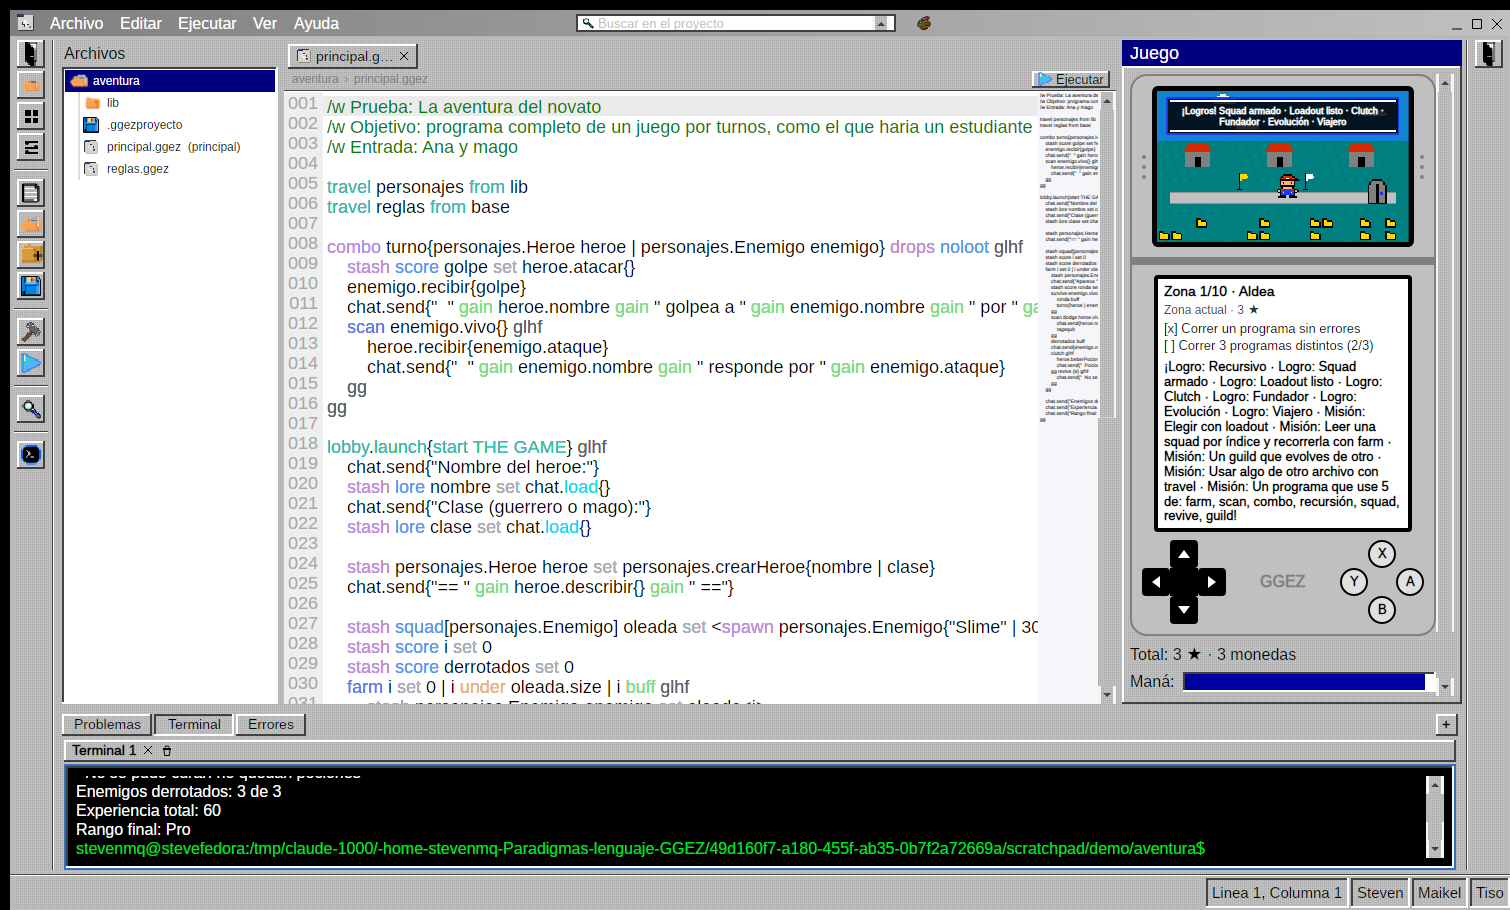
\includegraphics[width=\textwidth]{img/ide_ejecucion.png}
\caption{Ventana principal del IDE.}
\end{figure}

\begin{itemize}
  \item \textbf{Barra de menú} (arriba): Archivo, Editar, Ejecutar, Ver y Ayuda.
  \item \textbf{Barra lateral} (izquierda): íconos para cambiar entre el explorador de archivos, las extensiones y los ajustes.
  \item \textbf{Explorador}: el árbol de archivos del proyecto abierto.
  \item \textbf{Editor} (centro): pestañas con los archivos abiertos, números de línea, coloreado de sintaxis y minimapa a la derecha. Sobre el editor están la ruta del archivo y los botones de compilar (martillo) y ejecutar (reproducir).
  \item \textbf{Segmento de salida} (abajo): pestañas Terminal, Errores y Problemas.
  \item \textbf{Panel de juego} (derecha): maná, mapa del mundo, nivel actual, monedas, pistas y logros.
  \item \textbf{Barra de estado} (abajo del todo): línea y columna del cursor y otros datos.
\end{itemize}

El tamaño del explorador, del panel de juego y de la terminal se cambia arrastrando el divisor que los separa del editor; el divisor se resalta al pasar el mouse.

\manualseccion{Crear y abrir un proyecto}

\begin{enumerate}
  \item Menú \textbf{Archivo → Abrir carpeta} (\kw{Ctrl+O}) y elegir o crear una carpeta.
  \item En el explorador, clic derecho para crear archivos (\kw{.ggez}) y carpetas, renombrar o eliminar. Los archivos y carpetas que se crean, borran o editan fuera del IDE aparecen solos en el árbol, y una pestaña abierta sin cambios sin guardar se recarga con el contenido nuevo.
  \item Opcional: clic derecho sobre un archivo con \kw{lobby.launch} → \textbf{Marcar como principal}. El archivo aparece con la etiqueta «(principal)» y se usa cuando la pestaña enfocada no es un \kw{.ggez}.
\end{enumerate}

Sin proyecto abierto, también se puede crear un archivo suelto con \kw{Ctrl+N}, guardarlo y ejecutarlo.

\manualseccion{Escribir código}

\begin{itemize}
  \item El editor colorea palabras reservadas, tipos, operadores, textos y comentarios.
  \item \textbf{Autocompletado}: aparece al escribir o con \kw{Ctrl+Espacio}. Sugiere palabras reservadas, plantillas completas (por ejemplo, un \kw{farm} con sus tres partes) con su descripción, los nombres declarados en el archivo y, después de un punto, los miembros disponibles (\kw{chat.send}, \kw{lista.recruit}, lo de un módulo importado). Con las flechas se elige y con \kw{Enter} o \kw{Tab} se inserta; \kw{Esc} cierra la lista.
  \item \textbf{Minimapa}: muestra todo el archivo en miniatura a la derecha del editor; un clic salta a esa parte.
  \item Con la extensión de colores de bloques, al presionar \kw{Enter} después de \kw{glhf} el editor cierra el bloque con \kw{gg}.
  \item \kw{Ctrl+F} busca, \kw{Ctrl+H} reemplaza y \kw{Ctrl+G} va a una línea.
\end{itemize}

\begin{figure}[H]
\centering
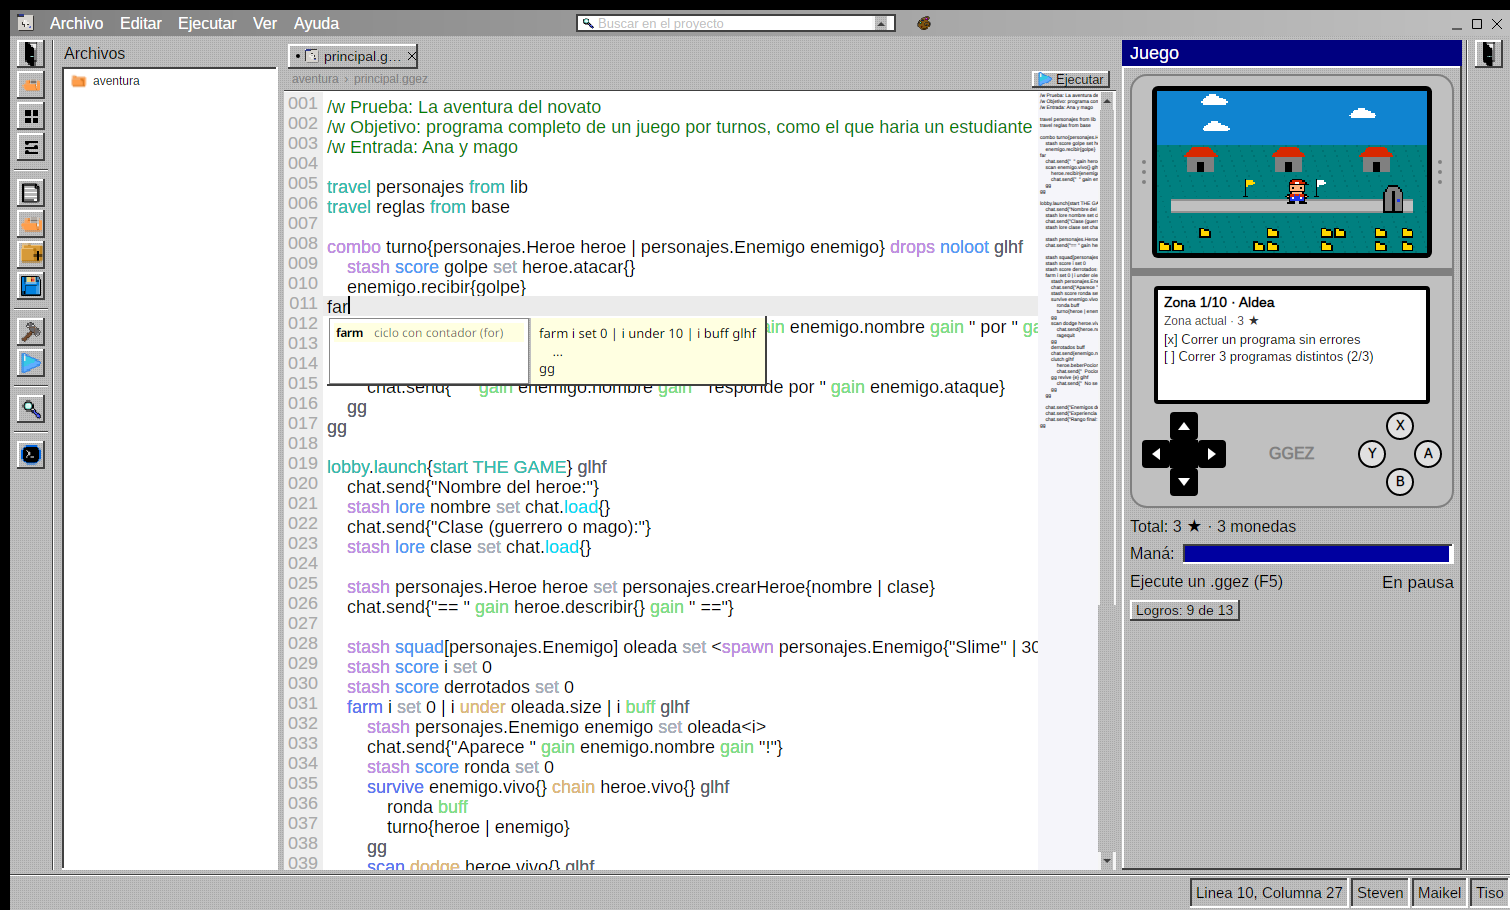
\includegraphics[width=0.92\textwidth]{img/autocompletado.png}
\caption{Autocompletado con plantillas y su descripción.}
\end{figure}

\manualseccion{Compilar y ejecutar}

\begin{itemize}
  \item \textbf{Compilar} (\kw{F6} o el martillo): revisa el archivo \kw{.ggez} de la pestaña enfocada sin ejecutarlo. Si todo está bien, la terminal muestra «Compilacion exitosa».
  \item \textbf{Ejecutar} (\kw{F5} o el botón de reproducir): compila y, si no hay errores, ejecuta el archivo \kw{.ggez} de la pestaña enfocada. Lo que imprime el programa aparece en celeste. Cuando el programa pide datos con \kw{chat.load}, se escriben en la terminal y se presiona \kw{Enter}.
  \item \kw{Ctrl+C} en la terminal detiene un programa en ejecución.
\end{itemize}

\manualseccion{Corregir errores}

\begin{enumerate}
  \item Si hay un error, la terminal lo muestra en rojo y la pestaña \textbf{Problemas} lo lista con su tipo, archivo, línea y posible causa.
  \item Un clic sobre el problema abre el archivo y lleva el cursor a la línea.
  \item Las advertencias aparecen en amarillo y no impiden ejecutar.
  \item Menú \textbf{Ejecutar → Ver errores} abre la pestaña de errores.
\end{enumerate}

\manualseccion{Terminal}

La terminal permite escribir comandos del sistema y tiene comandos propios: \kw{cd}, \kw{clear}, \kw{exit} y \kw{help}. Con el botón \textbf{+} se abren hasta cuatro terminales, una al lado de la otra. La primera terminal es siempre la terminal de \ggez, donde se compila y ejecuta. Con la extensión de Claude instalada, al escribir \kw{claude} en ella se abre otra terminal al lado con el asistente; en sus menús se elige con las flechas y \kw{Enter}.

Colores de la terminal: verde el indicador, blanco lo que escribe el usuario, celeste la salida del programa, rojo los errores y amarillo los avisos y advertencias.

\manualseccion{Modo de juego}

\begin{itemize}
  \item \textbf{Maná}: la barra muestra cuánto gastó el último programa.
  \item \textbf{Mapa}: muestra la zona actual y sus misiones; las flechas recorren las zonas. Al cumplir todas las misiones de una zona se abre la siguiente.
  \item \textbf{Niveles}: abrir la carpeta de un nivel (con \kw{nivel.json}) y ejecutar el archivo; el panel muestra cuántas pruebas pasaron y las estrellas ganadas.
  \item \textbf{Pistas}: el botón de pista gasta una moneda y muestra la siguiente pista del nivel.
  \item \textbf{Logros}: la lista muestra los obtenidos y los pendientes.
\end{itemize}

\manualseccion{Extensiones y ajustes}

En la vista de \textbf{Extensiones} se instalan y desinstalan complementos con un clic, entre ellos los temas desbloqueados con estrellas. En \textbf{Ajustes} se cambian el tamaño de letra, el zoom y otras preferencias del editor. Todo se conserva al cerrar el IDE, junto con las pestañas abiertas.

\begin{figure}[H]
\centering
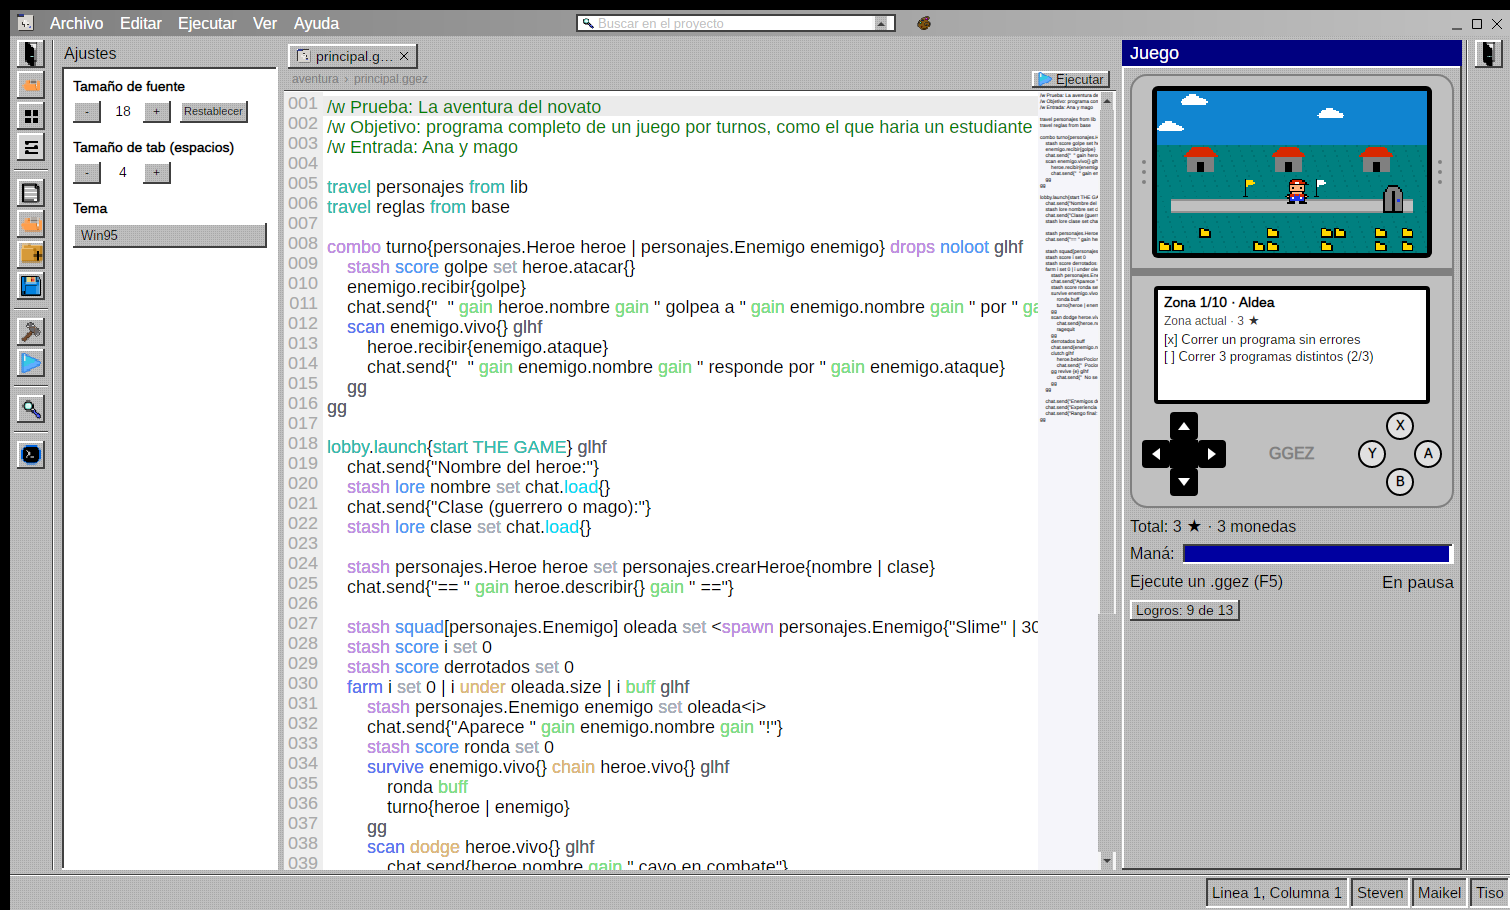
\includegraphics[width=0.92\textwidth]{img/ajustes.png}
\caption{Vista de ajustes.}
\end{figure}

\manualseccion{Ayuda}

\begin{itemize}
  \item \textbf{Ayuda → Sintaxis de GGEZ}: referencia completa del lenguaje, con cada ejemplo junto a su equivalente en Java.
  \item \textbf{Ayuda → Atajos de teclado} (\kw{F1}): lista de todos los atajos.
  \item \textbf{Ayuda → Acerca de}: versión e integrantes.
\end{itemize}

\begin{figure}[H]
\centering
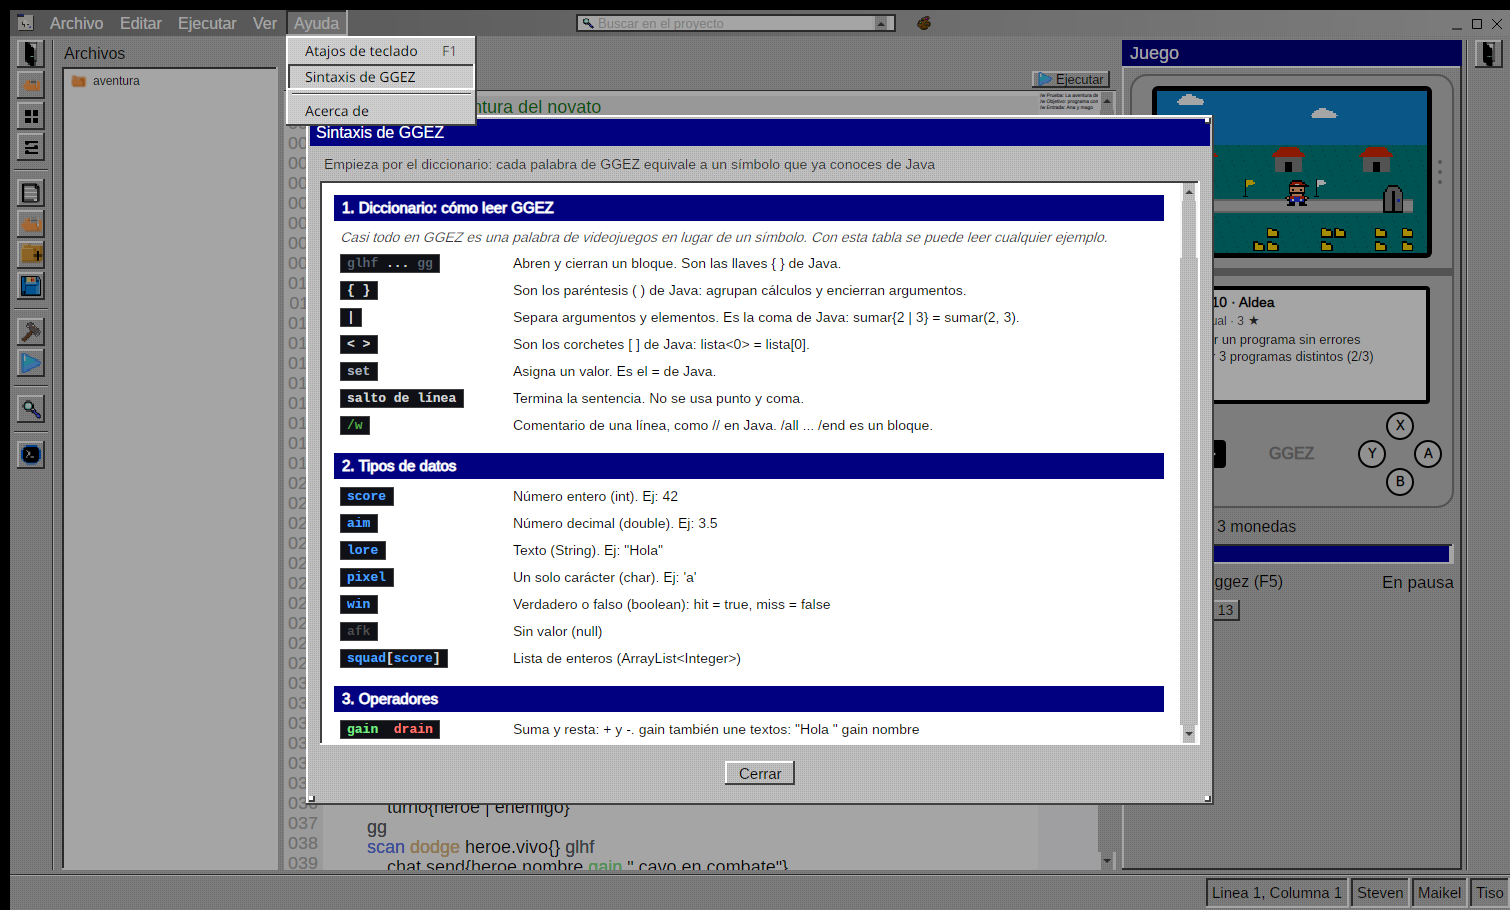
\includegraphics[width=0.92\textwidth]{img/sintaxis.png}
\caption{Referencia del lenguaje con el equivalente en Java.}
\end{figure}

\begin{figure}[H]
\centering
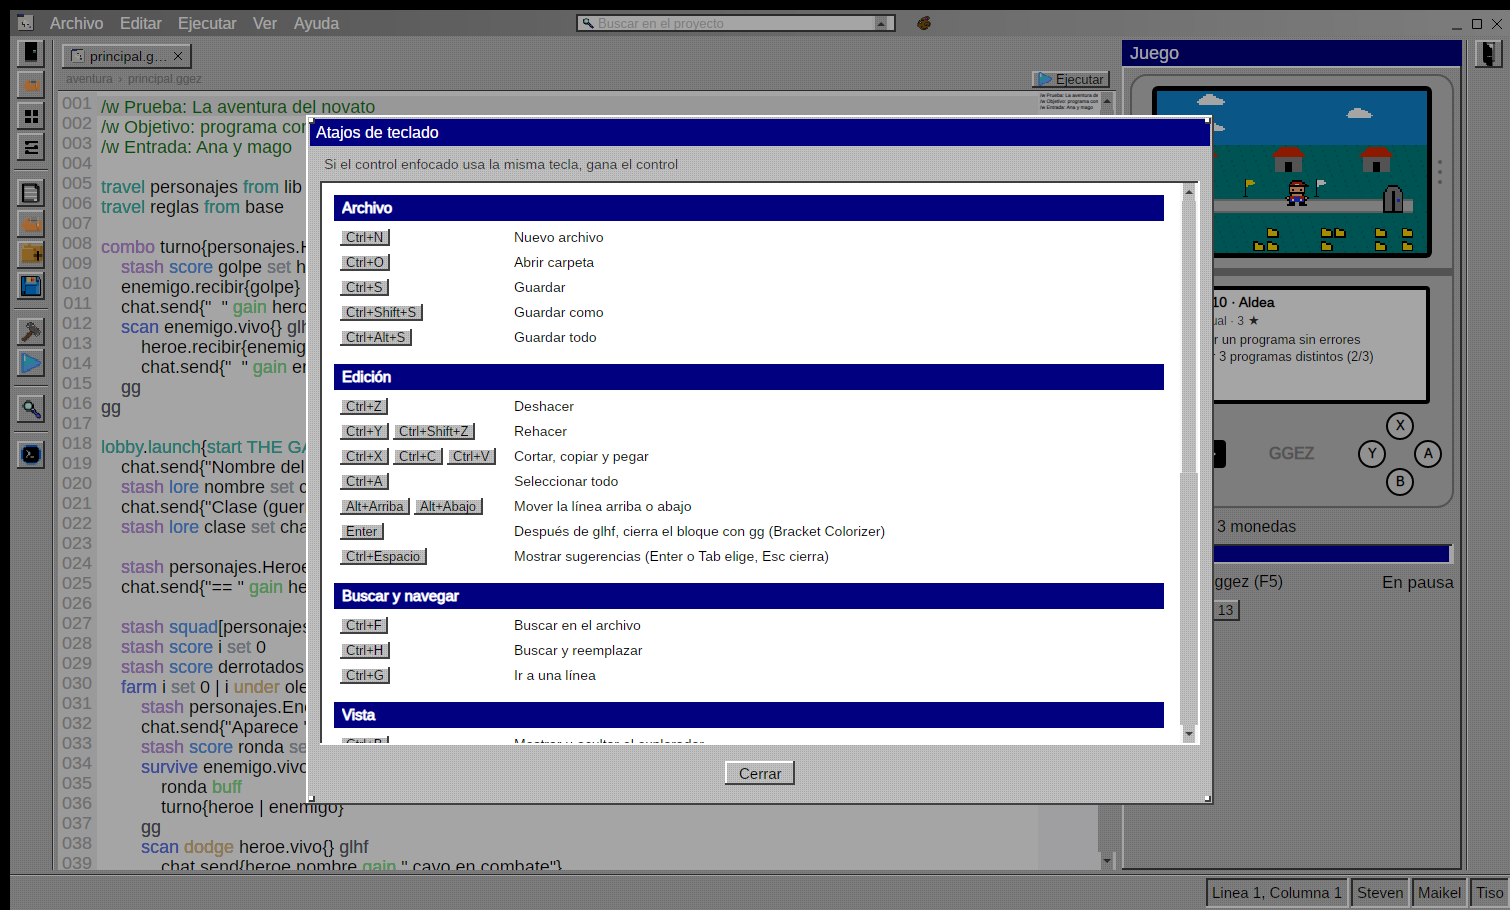
\includegraphics[width=0.92\textwidth]{img/atajos.png}
\caption{Atajos de teclado.}
\end{figure}

\manualseccion{Atajos principales}

\begin{longtable}{|p{5cm}|p{9.4cm}|}\hline
\cab\textbf{Atajo} & \textbf{Acción} \\\hline\endhead
\kw{F5} / \kw{F6} & Ejecutar / Compilar \\\hline
\kw{F1} & Mostrar los atajos \\\hline
\kw{Ctrl+N}, \kw{Ctrl+O} & Nuevo archivo, abrir carpeta \\\hline
\kw{Ctrl+S}, \kw{Ctrl+Alt+S} & Guardar, guardar todo \\\hline
\kw{Ctrl+Z}, \kw{Ctrl+Y} & Deshacer, rehacer \\\hline
\kw{Alt+Arriba} / \kw{Alt+Abajo} & Mover la línea \\\hline
\kw{Ctrl+Espacio} & Sugerencias de autocompletado \\\hline
\kw{Ctrl+F}, \kw{Ctrl+H}, \kw{Ctrl+G} & Buscar, reemplazar, ir a línea \\\hline
\kw{Ctrl+B}, \kw{Ctrl+J} & Mostrar u ocultar explorador y terminal \\\hline
\kw{Ctrl++}, \kw{Ctrl+-}, \kw{Ctrl+0} & Zoom \\\hline
\kw{Ctrl+C} (en la terminal) & Interrumpir el programa \\\hline
\end{longtable}



\end{document}
